\documentclass[journal]{vgtc}                % final (journal style)
%\documentclass[review,journal]{vgtc}         % review (journal style)
%\documentclass[widereview]{vgtc}             % wide-spaced review
%\documentclass[preprint,journal]{vgtc}       % preprint (journal style)
%\documentclass[electronic,journal]{vgtc}     % electronic version, journal

%% Uncomment one of the lines above depending on where your paper is
%% in the conference process. ``review'' and ``widereview'' are for review
%% submission, ``preprint'' is for pre-publication, and the final version
%% doesn't use a specific qualifier. Further, ``electronic'' includes
%% hyperreferences for more convenient online viewing.

%% Please use one of the ``review'' options in combination with the
%% assigned online id (see below) ONLY if your paper uses a double blind
%% review process. Some conferences, like IEEE Vis and InfoVis, have NOT
%% in the past.

%% Please note that the use of figures other than the optional teaser is not permitted on the first page
%% of the journal version.  Figures should begin on the second page and be
%% in CMYK or Grey scale format, otherwise, colour shifting may occur
%% during the printing process.  Papers submitted with figures other than the optional teaser on the
%% first page will be refused.

%% These three lines bring in essential packages: ``mathptmx'' for Type 1
%% typefaces, ``graphicx'' for inclusion of EPS figures. and ``times''
%% for proper handling of the times font family.

\usepackage{mathptmx}
\usepackage{graphicx}
\usepackage{times}
\usepackage{epstopdf}
\usepackage{amsmath}
\usepackage{multirow} 
\usepackage{amsmath}
\usepackage{color}

\usepackage{enumitem}

%% We encourage the use of mathptmx for consistent usage of times font
%% throughout the proceedings. However, if you encounter conflicts
%% with other math-related packages, you may want to disable it.

%% This turns references into clickable hyperlinks.

%\usepackage[justification=centering]{caption}

\usepackage[bookmarks,backref=true,linkcolor=black]{hyperref} %,colorlinks
\hypersetup{
  pdfauthor = {},
  pdftitle = {},
  pdfsubject = {},
  pdfkeywords = {},
  colorlinks=true,
  linkcolor= black,
  citecolor= black,
  pageanchor=true,
  urlcolor = black,
  plainpages = false,
  linktocpage
}

%% If you are submitting a paper to a conference for review with a double
%% blind reviewing process, please replace the value ``0'' below with your
%% OnlineID. Otherwise, you may safely leave it at ``0''.
\onlineid{0}

%% declare the category of your paper, only shown in review mode
\vgtccategory{Research}

%% allow for this line if you want the electronic option to work properly
\vgtcinsertpkg

%% In preprint mode you may define your own headline.
%\preprinttext{To appear in IEEE Transactions on Visualization and Computer Graphics.}

%% Paper title.

\title{AVIST: A GPU-Centric Design for Visual Exploration of Large Multidimensional Datasets  }

%% This is how authors are specified in the journal style

%% indicate IEEE Member or Student Member in form indicated below
%\author{Roy G. Biv, Ed Grimley, \textit{Member, IEEE}, and Martha Stewart}
%\authorfooter{
%% insert punctuation at end of each item
%\item
% Roy G. Biv is with Starbucks Research. E-mail: roy.g.biv@aol.com.
%\item
% Ed Grimley is with Grimley Widgets, Inc.. E-mail: ed.grimley@aol.com.
%\item
% Martha Stewart is with Martha Stewart Enterprises at Microsoft
% Research. E-mail: martha.stewart@marthastewart.com.
%}

%other entries to be set up for journal
%\shortauthortitle{Biv \MakeLowercase{\textit{et al.}}: Global Illumination for Fun and Profit}
%\shortauthortitle{Firstauthor \MakeLowercase{\textit{et al.}}: Paper Title}

%% Abstract section.
\abstract{
This paper presents  AVIST, an exploration oriented data visualization tool that  enables rapidly exploring and filtering large time-series multidimensional datasets on a commodity desktop computer.  AVIST highlights data exploration by gaining fine data details, which is achieved by animation and cross filtering interactions. To interactive visual exploration of big data, AVIST features a GPU-centric design.  Two key ideas are emphasized on the GPU-centric design: 1) data storage and computing are both on the GPU to fully utilize GPUs parallel computing and fast memory bandwidth; 2) a directed acyclic graph for characterizing data transformations on the GPU to support data aggregations and visualizations on users' demands. Based on the proposed designs, AVIST is implemented following the MVC pattern, and  focuses on 1) user interactions to slice big data into small  and 2) data transformations based  on the parallel computing. Lastly, two case studies are demonstrated that AVIST can help analysts identify abnormal behaviors and infer new hypotheses for visually exploring big datasets.}

%% Keywords that describe your work. Will show as 'Index Terms' in journal
%% please capitalize first letter and insert punctuation after last keyword
\keywords{Big data, interactive data exploration and discovery, multidimensional dataset}

%% ACM Computing Classification System (CCS). 
%% See <http://www.acm.org/class/1998/> for details.
%% The ``\CCScat'' command takes four arguments.

\CCScatlist{ % not used in journal version
 \CCScat{K.6.1}{Management of Computing and Information Systems}%
{Project and People Management}{Life Cycle};
 \CCScat{K.7.m}{The Computing Profession}{Miscellaneous}{Ethics}
}

%% Uncomment below to include a teaser figure.
%   \teaser{
%   \centering
%   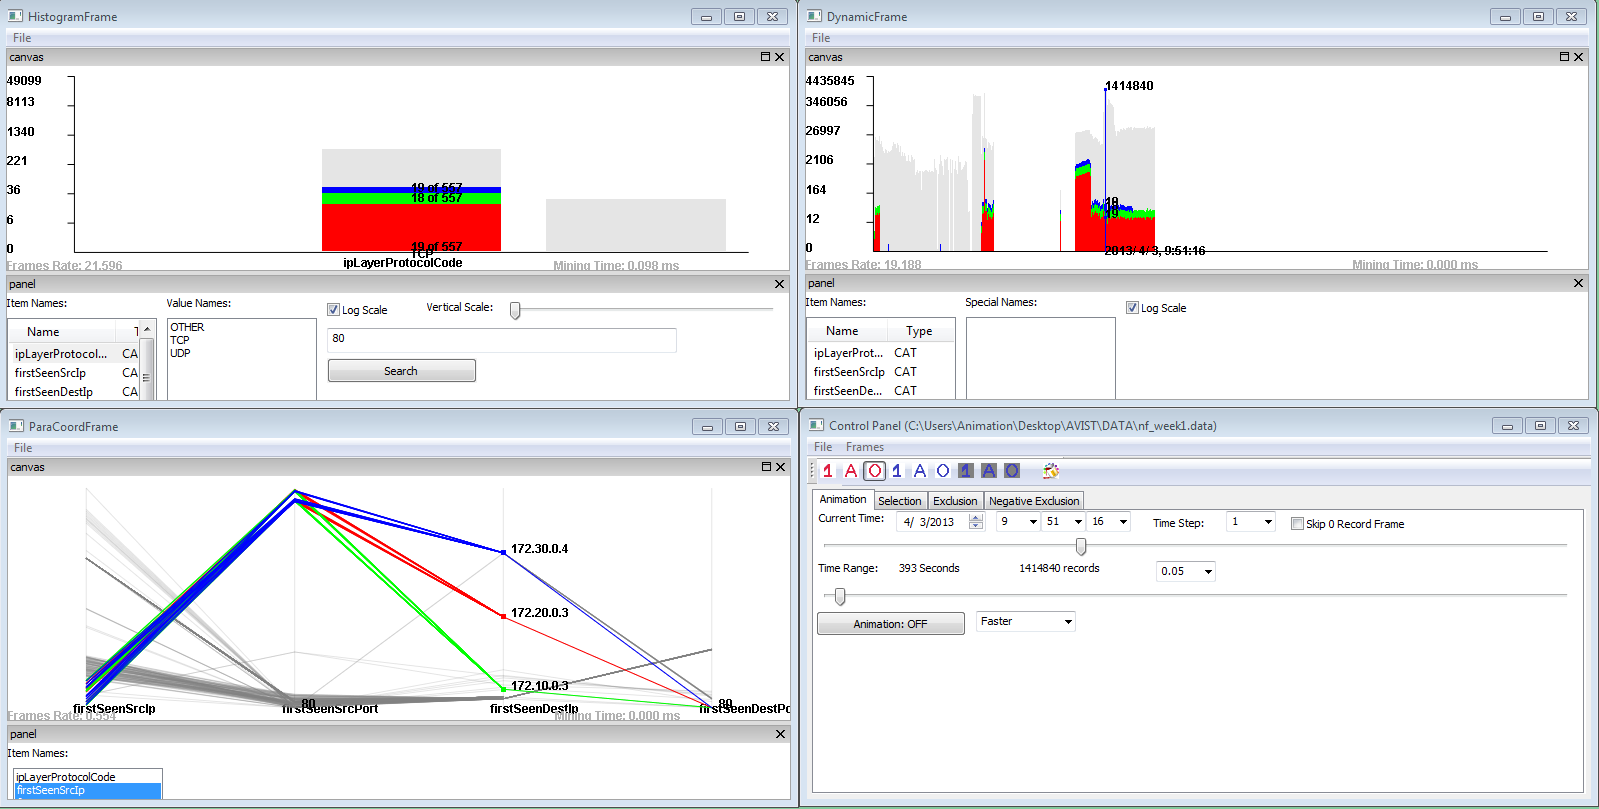
\includegraphics[width=16cm]{DataView.png}
   %	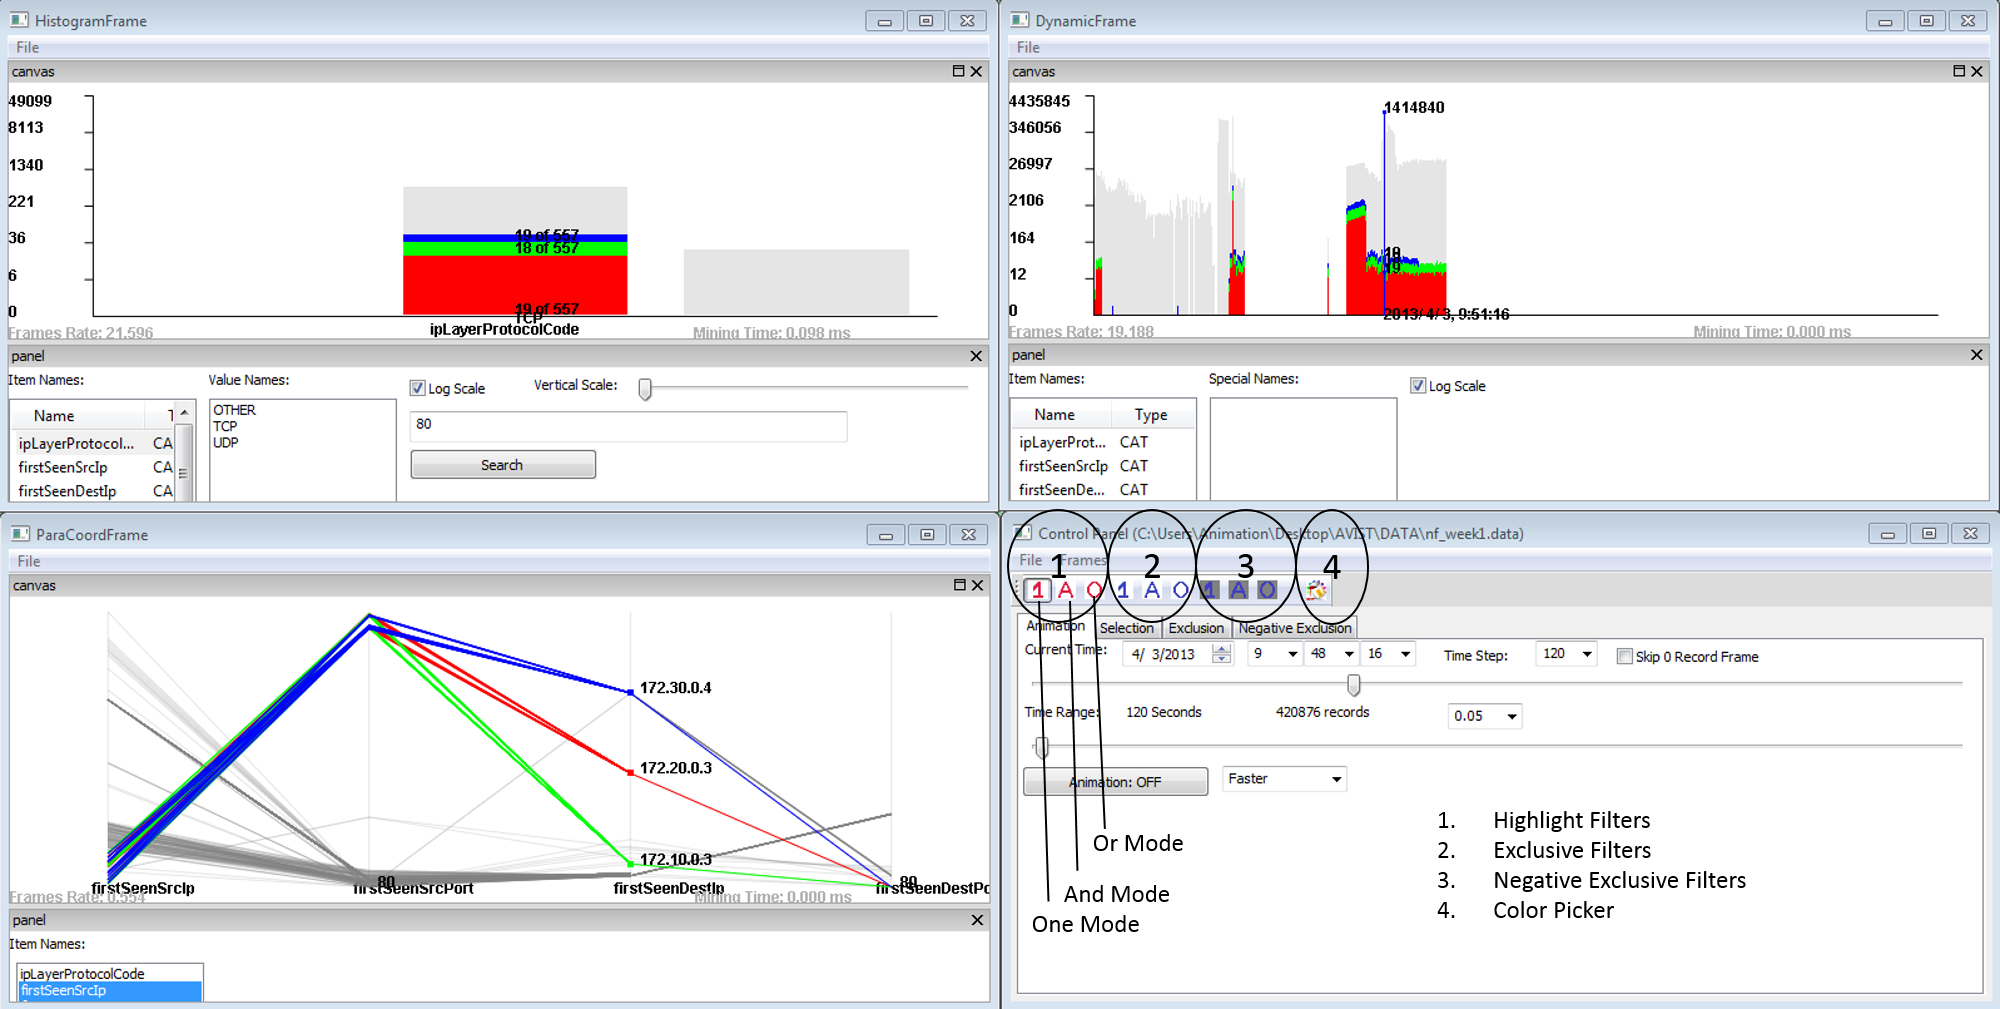
\includegraphics[width=1.0]{pic/DataView.png}
%   \caption{In the Clouds: Vancouver from Cypress Mountain.}
%  }

%% Uncomment below to disable the manuscript note
%\renewcommand{\manuscriptnotetxt}{}

%% Copyright space is enabled by default as required by guidelines.
%% It is disabled by the 'review' option or via the following command:
% \nocopyrightspace

%%%%%%%%%%%%%%%%%%%%%%%%%%%%%%%%%%%%%%%%%%%%%%%%%%%%%%%%%%%%%%%%
%%%%%%%%%%%%%%%%%%%%%% START OF THE PAPER %%%%%%%%%%%%%%%%%%%%%%
%%%%%%%%%%%%%%%%%%%%%%%%%%%%%%%%%%%%%%%%%%%%%%%%%%%%%%%%%%%%%%%%%

\begin{document}

%% The ``\maketitle'' command must be the first command after the
%% ``\begin{document}'' command. It prepares and prints the title block.

%% the only exception to this rule is the \firstsection command
\firstsection{Introduction}

\maketitle


As the rapid growing of data, interactive visual analysis becomes a key component to gain usable insights from massive data. To support sensemaking of big data, exploratory visual analysis emphasizes three aspects. Firstly, \textsl{flexible data filtering} (e.g., cross-filtering~\cite{ weaver2008, weaver2010}) empower analysts to ``prune" large datasets to gain buried relationships. Secondly, \textsl{fine data details} should be provided on demand, so that analysts can capture certain subtle abnormal activities. Lastly, \textsl{exploration data analysis} is usually an interactive and iterative process. Thus high performance is necessary for exploration of big data, which requires real-time frame-rates. For example, when cyber security analysts attempt to identify attacks from millions of records in network traffic logs, they have to filter data records by iteratively using different data attributes to finally narrow down to the suspicious records.  

However, there are many challenges to achieve these goals for analyzing big data.
 When the data becomes bigger, it cannot feed into memory or the computation speed cannot afford real-time performance. In order to feed more data into memory, Tableau~\cite{tab} highlights the Tableau Data Engine (TDE)~\cite{Wesley}. The TDE is a specialized column-oriented format, which has high data compression ratio (considering the repeating values in the columns) and can provide high level data aggregation information. To achieve fast visual querying of big data, imMens~\cite{2013-immens} utilizes the GPU parallel computing to improve performance. Firstly, it aggregates data into data tiles by data cube technique. Secondly, it uses WebGL for data processing and rendering on the GPU. However, both Tableau and imMens only consider visual exploring the high level data aggregation information of big data. To flexibly investigate fine-grained data details, such as identifying buried data relationships by complexity filtering, those methods cannot directly be applied, and new techniques need to be investigated.   

This paper tackles the visual exploration of big data problem,  and aims to help analysts  get the fine-grained details by exploratory visual analysis of big datasets. To achieve this, we propose an animated visualization tool - AVIST, which runs on a  commodity desktop computer for analyzing millions of multi-dimensional data records per second by leveraging the GPU resources. We emphasize ``\textit{animation}" in the context of time-series multidimensional datasets for identifying data temporal behaviors. The performance of AVIST is judged by FPS (frame per second), which emphasizes the high velocity feature. In summary, our key contributions in this paper as follows:

1) We propose a GPU-centric design for interactive visual exploration of big datasets, which emphasizes that data storage and computation are done by the GPU.

2) We design a data dependency graph for characterizing data transformations on the GPU, which supports data aggregation and visualization on demand.

3) We implement  AVIST following the GPU-centric design as a proof of concept. AVIST emphasizes  the  animation and cross-filtering interactions for slicing big data into small, and the GPU parallel computing for transforming raw data into visual primitives. 

4) We present two usage scenarios to demonstrate that  AVIST can help analysts identifying abnormal behaviors of large network flow and inferring new hypotheses for international trade transactions.     



\section{Related Work}

For visual exploration of big datasets, four questions outline the discussion of related work: 1) which type of data should be visualized, and what is the characteristic; 2) how to store and manage big data; 3) how to compute big data and achieve better performance; 4) how to explore and interact with big data.

\subsection{The Exploration of Multidimensional Datasets}
Large multidimensional datasets are very common and ubiquitous. Most of them are usually behavioral data that are generated by people or machines, which have a natural temporal ordering (streaming data)~\cite{Canny}. Besides the large volume,  high velocity is also an important consideration for analyzing such multidimensional datasets~\cite{IBM2011}. For example, network logs and financial transactions can be generated millions per second. When faced with large volume and high velocity multidimensional datasets, analysts may not know what they are looking for; they will know something is interesting only after they find it. In this setting,  analysts have no idea how to formulate their queries. Thus, the data exploration of large time-series and multidimensional datasets is the key ingredient for knowledge discovery~\cite{harvard}.

The exploration driven system for knowledge discovery becomes a novel requirements in the era of ``Big Data". The data exploration becomes a first class for making sense of large streaming multidimensional datasets. Our paper tackles this problem and provides a solution for building an exploration oriented tool by considering the large volume and high velocity datasets.
%handling big data considering: 1) the volume of data (length of data); 2) the velocity of data (speed of data); 3) the attributes of data (width of data). 

\subsection{Big Data Management}
The data management methods vary based on the size of datasets. If a dataset can fit into the computer memory,  the data layout methods and data structure design should be investigated. When a dataset size is larger than the computer memory capacity, data prefetching and out-of-core techniques need considered~\cite{OFC}. If a dataset is even bigger than the computer disk capacity, the distributed file systems such as HDFS (Hadoop Distributed File System)~\cite{HDFS} can be a choice. 

This paper aims to achieve real-time performance for visual exploration of big data on a commodity desktop. Thus it only considers that datasets can fit into the computer memory. Previous researches, such as  imMens~\cite{2013-immens}, use one million or more data items as a threshold. Thus, this paper follows this definition and gives an upper bound of  big data: the capacity of the computer memory.

To manage big data, especially the multidimensional (tabular) datasets, on computer memory, there are two general ways: row oriented format and column oriented format. Abadi et al.~\cite{Abadi:2008} discussed the differences between these two methods, and pointed out that column format can apply compression techniques to significantly reduce data size and improve query performance. For example, Tableau's TDE is based on column oriented format for managing big data.

Data modeling, sampling and aggregation~\cite{2013-immens} are other ways for handling big data. These methods reduce big data into small size based on data precomputations. However, these kinds of  visual explorations are constrained by precomputation methods, and cannot afford flexibility and low level data details. Our paper emphasizes  visual exploration data fine-grained details by complex filtering and highlighting. Thus, we manage the big multidimensional datasets in row oriented format, and utilizes parallel computing for visual exploration of big data on demand. %Section 3 gives more discussion about it.

\subsection{The GPU Acceleration}

Contrasted with CPUs, graphics processing units (GPUs) have two unique features.

\begin{itemize}
	\item More cores and fine levels of parallelism. GPUs are many-core architecture, which may have thousands of cores.  This feature makes the GPUs  specialized compute-intensive, highly parallel computation. 
	\item Higher memory bandwidths. This means that  GPUs can access data in a fast way (usually more than 100GB/s), or more data in a fixed time period.
	%	\item Weak data cache and flow control. GPUs lack of complexity cache organization and sophisticated branch predication.
\end{itemize}

GPUs are more popular in scientific computing and visualization~\cite{volume}, and several factors have hampered them as general-purpose computing in information visualization and visual analysis fields. Primarily GPUs lack of complexity cache organizations and sophisticated branch predications, which makes the complicated sequential algorithms hard to be parallelized on the GPU platform. In fact,  the development of GPU libraries (e.g., Thrust and cuBLAS) lowers the bar for transforming these algorithms to the GPU platform. Another consideration is slow transfers from CPU to GPU memory, and the limited GPU memory size. However, transfer speeds have improved significantly thanks to PCI-bus improvement, and now the GPU memory capacity is quite good (the latest Nvidia Geforce GTX TITAN Z has 12GB memory).  All these GPU developments make it as a possible solution for handling big data to support exploratory data analysis~\cite{Pawliczek}. 

In fact, GPUs have a deep root in graphics and visualization, and they are good at handling million of pixels. This paper aims to utilize GPUs' fine computing parallelism and high memory bandwidths to support exploratory visual analysis of large multidimensional datasets. Thus, we propose AVIST, which is an animated visualization tool, implemented based on a GPU-centric design for visually exploring big time-series and multidimensional datasets. 

\subsection{Big Data Exploration}
Querying is one of the fundamental interaction techniques for exploring data. Polaris~\cite{polaris} features a visual querying language by integrating analysis and visualization of multidimensional datasets. Analysts can construct sophisticated visualizations by simple drag-and-drop operations. However, Polaris is incapable of managing big data. Tableau, the successor of Polaris, makes a big progress for the big data visualization.  whereas it lacks flexible visual filtering for investigating data details.

Animation is a kind of time multiplexing technique~\cite{Fekete} for visualizing large data items. Moreover, it can effectively reveal temporal patterns by significantly improving graphical perception~\cite{animated}. This paper highlights animation interactions for slicing big data into details. Cross-filtering~\cite{weaver2010} is a method for flexible visually drilling-down into fine-grained relationships for multidimensional datasets. Hence we emphasize cross-filtering and utilize the GPUs to improve performance, to achieve fast, flexible and detailed data exploration. 



 \section{The GPU-Centric Design}
\subsection{Design Principle}
The design of AVIST follows two important principles: 1) \textit{fully utilizing the GPU  fine parallelism and high memory bandwidth to boost performance on a commodity desktop computer}; 2) \textit{affording flexible visual querying and filtering, such as animation and cross-filtering, to visually explore fine level data details}. Based on these two guidelines, we carefully consider the data storage and computation design on the GPU:
\begin{itemize}
\item  \textbf{Data storage}:  We store  raw data on the GPU memory. Moreover, all derived data are also on the GPU memory to fully take advantage of the GPU high memory bandwidth.


\item \textbf{Data computation}: We highlight cross-filtering  for slicing data records from different attributes (animation for time domain). A data dependency graph (directed acyclic graph) characterizes such data transformations on the GPU to support data aggregation and visualization on demand.

\end{itemize}

\subsection{The GPU-Centric Design}

There are two key ideas about the GPU-centric design: 1)  raw data is stored on the GPU memory; and 2) data processing is parallelized on the GPU.

We emphasize that the raw data is important for exploratory visual analysis. Because it can potentially help analysts to analyze each data record without any information loss (\textit{finding a needle in haystack}).  The raw data is stored in the GPU memory, which enables: 1) fast data accessing based on its high bandwidth; and 2) avoiding data transfers between CPU and GPU. Besides the raw data,  the derived data is also stored on the GPU memory (visual primitives are stored on the GPU vertex buffer objects). 

We also highlight that data aggregation and visualization are  based on the GPU parallel computing. The benefits include: 1) vectored computing for utilizing the GPU fine level parallelism; 2) data aggregations  and visualizations are on demand rather than precomputation.


\begin{figure}[htb]
	\centering
	
	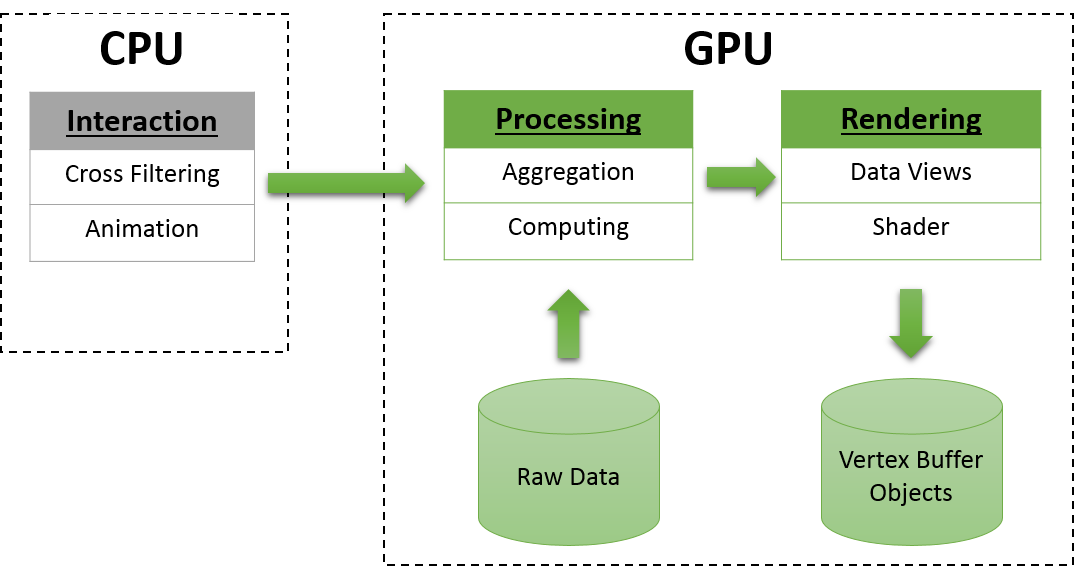
\includegraphics[width=1.0\linewidth]{pic/arch.png}
	\parbox[t]{1.0\columnwidth}{\relax
	}
	%
	\caption{\label{fig:architecture} The GPU-centric design: user interactions are transfered from the CPU to the GPU. Data storage and computation are on the GPU. }
\end{figure}


Figure~\ref{fig:architecture} shows the GPU-centric design. User interactions are generated in the CPU side, then they are transfered into the GPU, which triggers the GPU parallel processing and rendering.
The GPU is the main platform for data storage and  computing. 
The data resides on the GPU memory for fast fetching, which are mainly about raw data and visual primitives.  The GPU computation is also separated into two parts: 1) the general data aggregation and filtering; 2) the computation of each data view for generating visual primitives.  
%The GPU parallel computing is on the fly,  which is caused by user interactions (animation and cross filtering).  
In all, the GPU-centric design emphasizes that both data storage and processing are handled by the GPU, which fully utilizes the GPU  parallelism and high memory bandwidth.

\subsection{Data Storage}
As we mentioned, the GPU memory capacity limits the GPU-centric design for handling even larger datasets.  To feed more data into the GPU memory, we apply a lossless compression technique for preprocessing  multidimensional datasets. 

  

Consider a multi-dimensional dataset, which may include different types of data.  Firstly, we identify each data type, which can be separated into time data, quantitative data, and categorical-ordinal data. Secondly, we use different methods for compressing those types of data based on their characteristics.    
Considering the categorical-ordinal data, we count  all possible values and map each value into a unique ID. This  key-value map is stored in main memory as meta data.  We calculate the minimum and maximum values for time and quantitative data, and store them in main memory as  meta data.    
 
On the GPU side, we organize the raw data in a row-oriented format, where all data records are ordered by their time values (we emphasize the data temporal and spatial locality for fast data retrieving and processing). We store each data item's binary code instead of its ASCII code for saving memory space. Thus, each time data item occupies 8 bytes; each quantitative data needs 4 bytes (one \textit{Int} or \textit{Float}). We store categorical-ordinal data IDs instead of their values. The memory requirement of this type of data varies based on its possible values (one byte is needed if the number of possible values is less than 256; two bytes are considered if the number is less than 65536; other cases use four bytes). Table \ref{preprocessing} summarizes the compression methods for preprocessing datasets. %Considering a standard commercial graphics card with 4GB memory. If each data record have 10 dimensions and each item needs 4 bytes, then 100 million records can be stored on GPU memory theoretically.  
%Thus, one commodity-level GPU is capable for 100 million records dataset. 


\begin{table}[h]
	\centering
	\caption{Data Preprocessing Compression}
	\label{preprocessing}
	\begin{tabular}{|c|c|c|}
		\hline
		\textbf{DataType}                                                     & \begin{tabular}[c]{@{}c@{}}\textbf{GPU memory}\\ \textbf{binary format}\end{tabular} & \begin{tabular}[c]{@{}c@{}} \textbf{Main memory} \\ \textbf{meta-data}\end{tabular}   \\ \hline
		Time                                                         & \begin{tabular}[c]{@{}c@{}}time\_t\\ 8 bytes\end{tabular}          & \begin{tabular}[c]{@{}c@{}}minimum value\\  maximum value\end{tabular}         \\ \hline
		Quantitative                                                 & \begin{tabular}[c]{@{}c@{}}Int or Float\\  4 bytes\end{tabular}    & \begin{tabular}[c]{@{}c@{}}minimum value\\ maximum value\end{tabular}         \\ \hline
		\begin{tabular}[c]{@{}c@{}}Categorial-Ordinal\end{tabular} & $1\sim4$ bytes                                                          & \begin{tabular}[c]{@{}c@{}}Dictionary\\ (IDs and data values)\end{tabular} \\ \hline
	\end{tabular}
\end{table}

 Compared with the row-oriented format, the column-oriented data organization has better performance on some analytical workloads.  However, we use row-oriented format instead of column-oriented by considering several factors: 1) exploratory analysis cares more about fine-grained record details rather than high level aggregations, and we want to guide the analysts to each data record based on their querying and filtering, rather than showing them high level aggregation information; 2) column-oriented format primarily works on columns, which are treated individually. Thus, queries for each column works efficiently, while cross-column queries need to retrieve multiple columns and to assemble those data in a complex way. The computation may be very heavy and cannot easily be vectorized; 3) the row-oriented data has the spatial locality based on its IDs. If the data has time,  temporal and spatial locality can be unified together for fast data retrieving; 4) the computation of row-oriented data can easily be vectorized by leveraging GPU fine parallelism to improve performance.
 
 \subsection{Data Computation}       

To organize the parallel computing of GPUs, a data dependency graph is proposed to characterize the data transformations. Figure~\ref{fig:datagraph} shows the detailed data flow design, which is a kind of directed acyclic graph. In this figure,  rectangles represent the data, while ovals are the parallel computations. The graph can be separated into three parts:

\begin{figure}[htb]
	\centering
	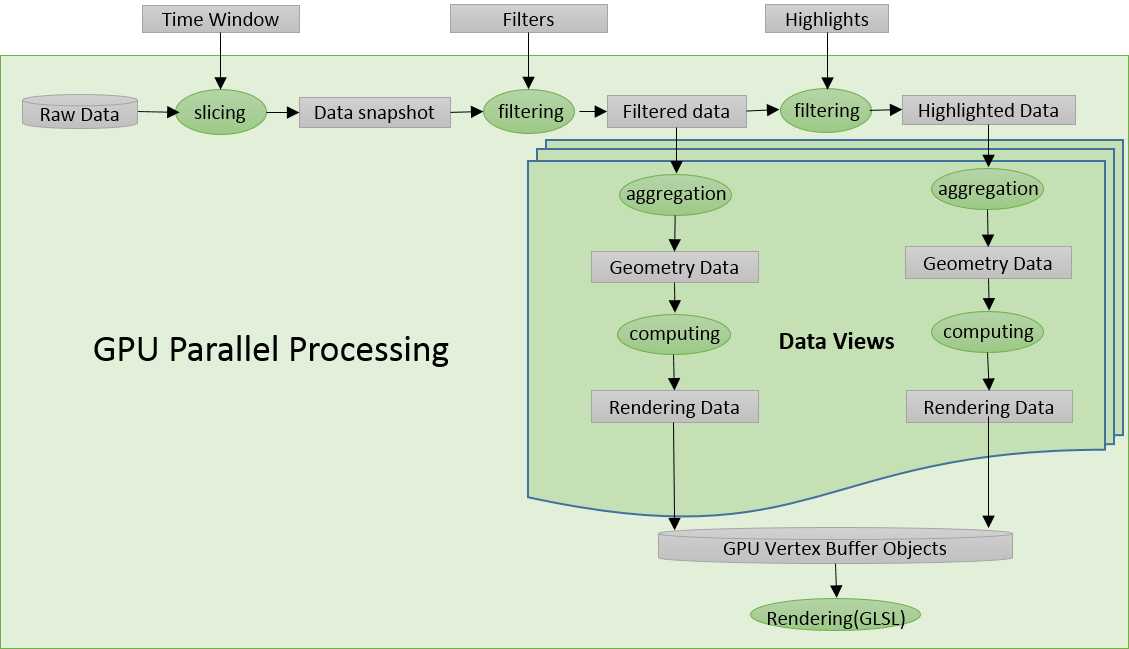
\includegraphics[width=1.0\linewidth]{pic/flow-chart.png}
	\parbox[t]{1.0\columnwidth}{\relax
	}
	%
	\caption{\label{fig:datagraph} The data dependency graph: rectangles represent the data and ovals are the parallel computations. Data filters are generated in the CPU side and transformed to the GPU. All data and computations are done on the GPU. } 
\end{figure} 

\begin{itemize}
	\item \textbf{Data filtering}. Data filters (e.g., \textsl{time window}, \textsl{filters} and \textsl{highlights}) are generated by user interactions in the CPU side, then they are passed to the GPU side.  The GPU pipeline of data filtering is as follows. Firstly,  time window is applied to slice the raw data into data snapshots. Secondly,  filters are applied to data snapshots by removing uninteresting data records. Lastly, highlights  aim to emphasize important data items from the filtered datasets.  
	\item \textbf{Data processing}. The aim of this step is to transform the filtered data records into visual primitives. However, data transformation methods varies considering different data views. We summarize them and character data processing into two stages for each data view: 1) aggregation for generating geometry data (e.g., binning data for histogram view); 2) computation for transforming geometry data into visual primitives  (e.g., the bar height for histogram view).
	\item \textbf{Data rendering}. All generated visual primitives are stored in GPU vertex buffer objects. GLSL (OpenGL shading language) codes generate the ultimate visual results when rendering the visual primitives on the screen (e.g.,  splitting one vertex into four for rendering rectangles by geometry shader,  filling colors in triangles by fragment shader). 
\end{itemize}	
 

 


The data dependency graph has several advantages. Firstly, it follows the cross-filtering design pattern~\cite{weaver2010cross}, where the cross-filtering and coordinated multiple view are coupled together.
Secondly, all data processing and visual rendering can easily be vectorized, and data computations are on the fly. Thirdly,  incremental computing can be applied to exploit temporal and spatial locality. When users play animation, frame-to-frame coherence can be exploited. In such cases, only incremental data need to be considered. Moreover, user interactions are  incremental and interactive. So previous querying results can be reused by next queries. Lastly, the data dependency graph is flexible and extensible. More data filters and data views can easily be extended.
%In all, we formalize the computation flow as a direct acyclic graph (DAG) on the GPU, which is the core part of the GPU-centric design.


~~~~~~~~~~~~~~~~  



 
 \section{AVIST}
We implemented an animated visualization tool (AVIST) based on the GPU-centric design.
AVIST is written in C++, its computation codes are based on CUDA 7.5 and visualization codes are based on OpenGL and GLSL. The interface are coded by wxWidgets. We use the Thrust library\footnote{https://developer.nvidia.com/Thrust} for accelerating sort, scan, transform and reduction operations.

 

In this section, we give the implementation details of AVIST from four aspects: 1) the code organization of AVIST, which follows the Model-View-Controller (MVC) pattern and separates the system into three aspects: data transformations (model), data views and data filters (control); 2) data transformations, which feature the GPU parallel computing to achieve better performance; 3) correlated data views, which provide different visual aspects of multidimensional datasets; 4) user interactions, which emphasize  animation and cross-filtering for slicing big data into small.

\subsection{MVC Pattern}
The codes organization of AVIST follows the Model-View-Controller (MVC) design pattern as shown in Figure~\ref{fig:mvc}. The filters belong to the control part, which directly are applied to data views shown as the dash lines. The solid lines describe the method invocations. Firstly, filters trigger data models. Then, the data views are updated after the data model's change, thus they give users visual feedbacks.

\begin{figure}[htb]
	\centering
	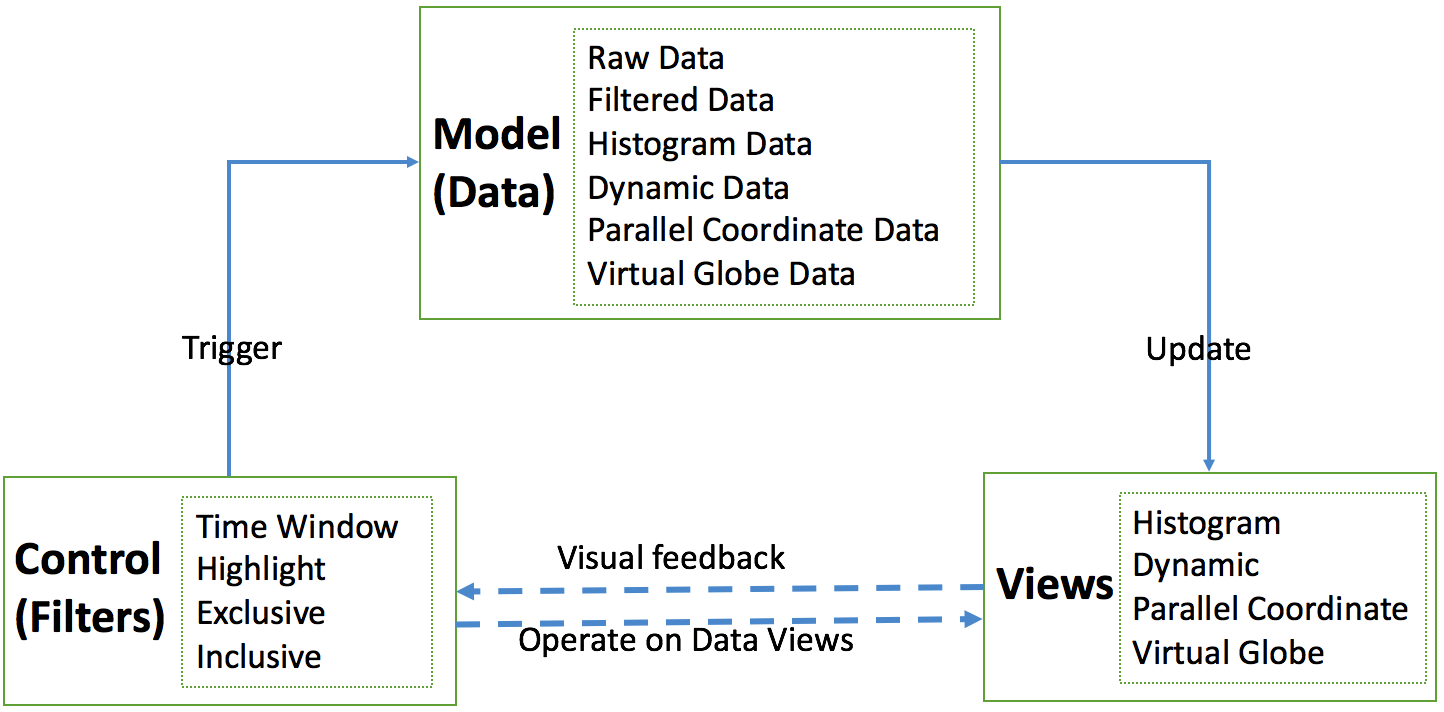
\includegraphics[width=1.0\linewidth]{pic/mvc.png}
	\parbox[t]{1.0\columnwidth}{\relax
	}
	%
	\caption{\label{fig:mvc} This figure shows the MVC design of AVIST. The dash lines show the visual operations and feedbacks between user interactions and data views. The solid lines describe the data path. First, filters trigger data model , then update the data views.  }
\end{figure}    


The MVC design pattern has several benefits. 1) We separate filters, data and views, which makes AVIST flexible to extend more filters, data transformations and data views in future.  2) The model part is implemented on the GPU, which highlights the GPU-centric design. 3) The cross-filter design pattern can easily be  applied. User interactions of one data view can update the filters, which triggers the data transforms and updates other data views.


\subsection{Data Transformation}
AVIST features the GPU based vectorized data transformations. In this section, we describe data transformations following the data dependency graph design: data filtering, data processing and data rendering.

\subsubsection{Data filtering} 
This stage describes data transformations from raw data into filtered data as shown in Figure~\ref{fig:dataTran1}.
Firstly, a time window slices the raw data into a data snapshot, then data  filters are applied to the data snapshot to remove uninteresting records or highlight important ones. To boost performance, a binary search is applied for slicing data based on the data temporal locality.  The sliced data records are checked by data filters in parallel, and then they are reduced to the filtered records.   

\begin{figure}[htb]
	\centering
	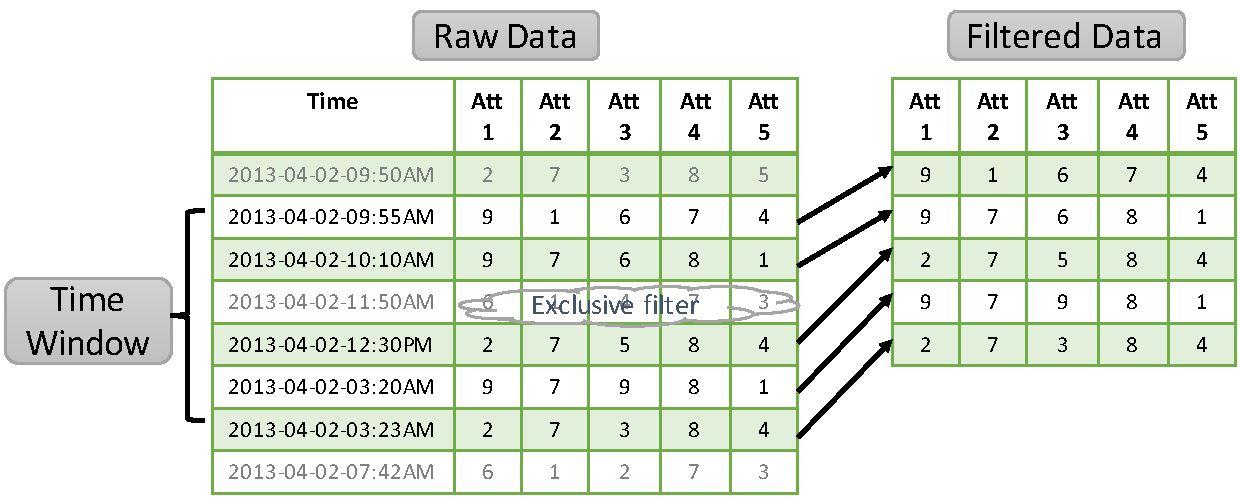
\includegraphics[width=1.0\linewidth]{pic/trans.pdf}
	\parbox[t]{1.0\columnwidth}{\relax
	}
	%
	\caption{\label{fig:dataTran1} Data transformations from raw data to filtered dataset.}
\end{figure} 




\subsubsection{Data processing}
The computations of data processing and rendering are view dependent. We demonstrate the detailed implementation of four data views: histogram view, time-series view, parallel coordinate plots and virtual global view (the descriptions of them are provided in section 4.3).

\begin{figure}[htb]
	\centering
	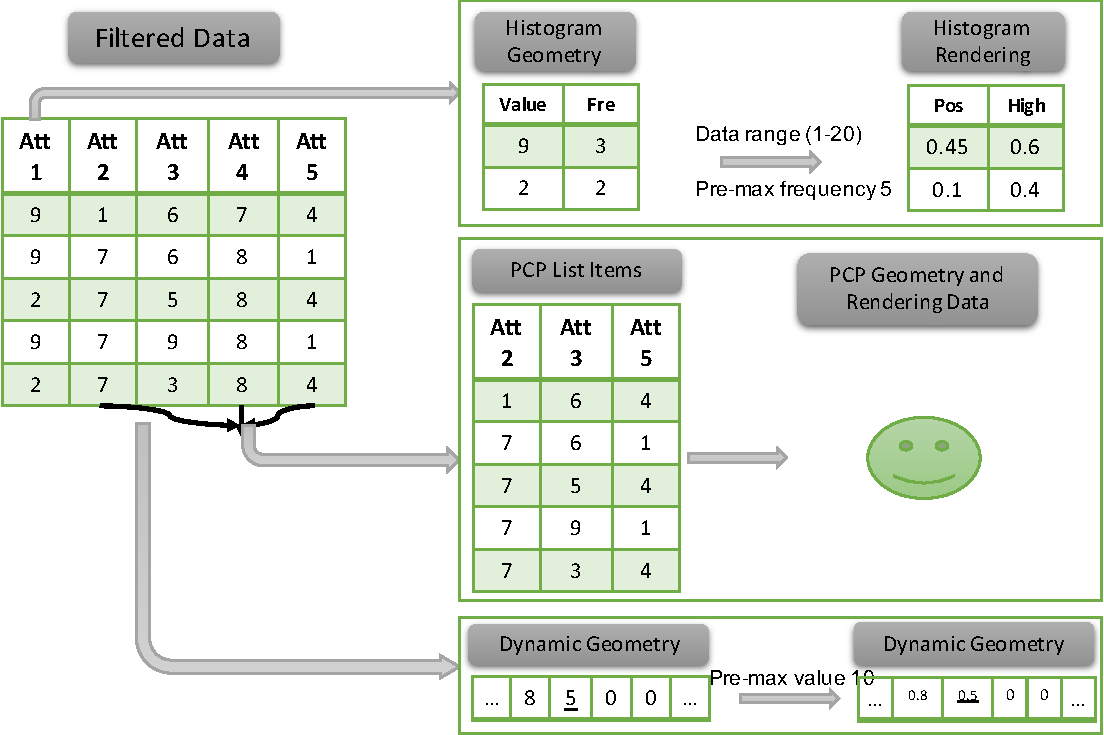
\includegraphics[width=1.0\linewidth]{pic/tran2.pdf}
	\parbox[t]{1.0\columnwidth}{\relax
	}
	%
	\caption{\label{fig:dataTran2} Data transformations from filtered data into visual primitives.}
\end{figure} 


\begin{figure}[htb]
	\centering
	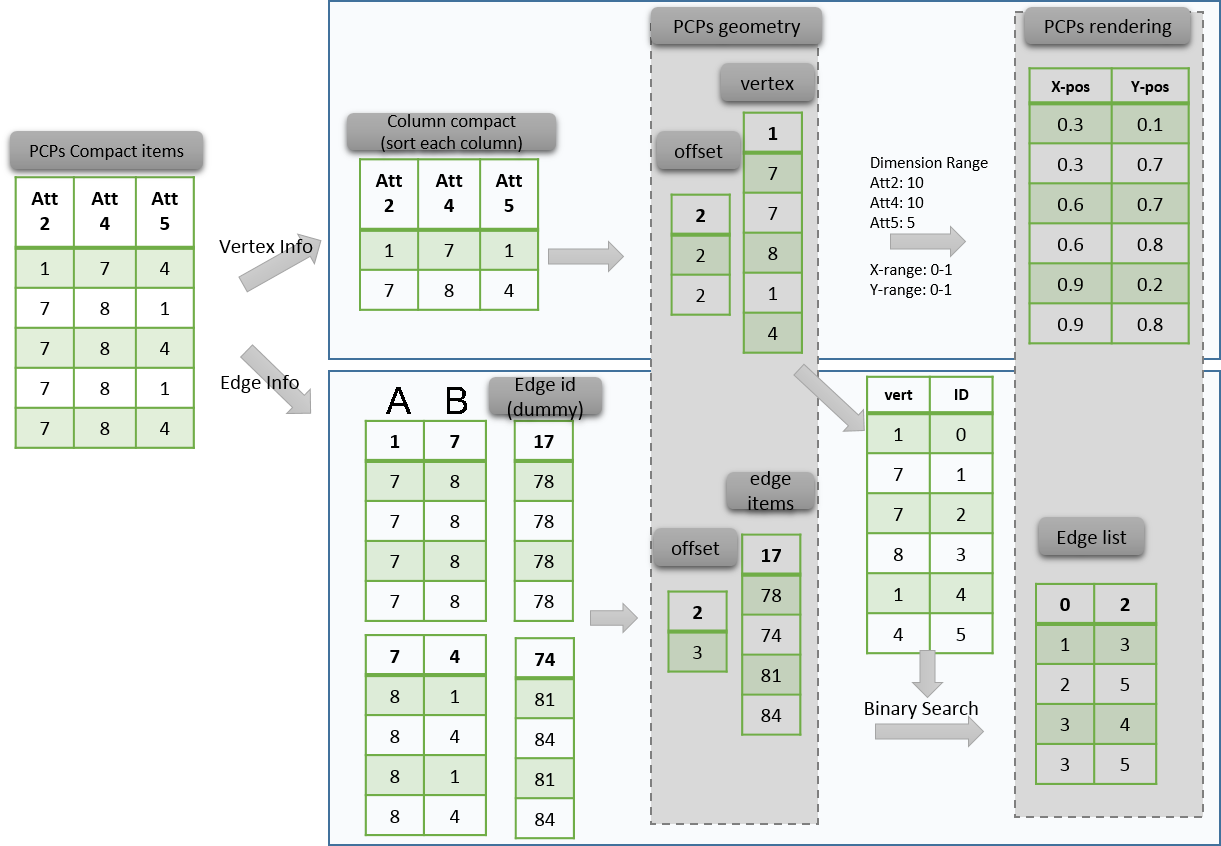
\includegraphics[width=1.0\linewidth]{pic/trans3.pdf}
	\parbox[t]{1.0\columnwidth}{\relax
	}
	%
	\caption{\label{fig:dataTran3} This figure shows data transformations from compact item lists to rendering data in parallel coordinate views. The data transformations are separated into two parts: vertex and edge.}
\end{figure} 

Figure~\ref{fig:dataTran2} demonstrates data transformation of histogram and dynamic views. Based on the users' chosen column, AVIST retrieves this column data,  aggregates them, and visualizes them. The steps are described as follows. 
\begin{enumerate}[noitemsep]
	\item Sort the  column to obtain unique values and their frequency.
	\item Get X position of each unique value based on the data range.
	\item Get Y position of each unique value based on previous maximum frequency.
\end{enumerate}	

Data transformations of  time-series view is straightforward: the GPU counts the number of  filtered data items, then transform it to height value (based on previous maximum value). 

Data transformations of parallel coordinate plots (PCPs) are more complex than other views. After the GPU generates PCPs compact items based on chosen axes, the data flow is separated into two parts as shown in Figure~\ref{fig:dataTran3}. The steps for generating vertex of PCPs:
\begin{enumerate}[noitemsep]
	\item  Sort each column to obtain unique values.
	\item Compact each column unique values into \textit{vertex} array with their size \textit{offset} array.
	\item Generate Y-axis positions based on the data dimensions' range, and X-axis positions based on the axis chosen order. 
\end{enumerate}

The steps for generating edge list of PCPs are as follows:
\begin{enumerate}[noitemsep]
	\item Two neighboring columns are grouped into one array, which is \textit{Edge ID} list. The values of list are called dummy values and calculated by: 
	
	$dummyValue = value_{columnA}*range_{columnA} + value_{columnB}$
	
	\item  Sort \textit{Edge ID} lists to obtain unique values.
	\item Compact each list unique values into \textit{edge} array with their size \textit{offset} array.
	\item Split \textit{edge} array into two arrays with vertex values of their columns.
	\item Replace vertex values with their orders based on \textit{vertex} array.
	
\end{enumerate}

The virtual global view is a special case of parallel coordinate views with two axes. The difference is that vertex position is 3D in virtual global view. And there are extra steps for generating 3D positions based on longitudes and latitudes. 
The lines are Bezier curves, which are generated based on virtual globe size and the strategies of selecting control points.


\subsubsection{Data rendering}
After generated visual primitives, AVIST maps them into the GPU vertex buffer objects. The  GPU VBOs offer substantial performance gains and avoids data transformations between main memory and GPU memory.

However,  visual primitives in VBOs are vertexes and edges. In order to  generate rectangles, areas or more advanced shapes, we use GLSL for post-processing. For example, we split one vertex into four vertexes to generate rectangles in histogram view. We also transform vertexes into line strip to generate areas in time-series view.


\subsection{Correlated Data Views}
Four data views are implemented in AVIST, which can provide different visual aspects of the multidimensional datasets.

\begin{itemize}
	
	
	\item \textbf{Histogram view} shows  data distribution of  sliced data snapshot. Analysts can select different dimensions  from a listbox to explore different aggregation information.
	
	\item \textbf{Time-series view} shows the data aggregation of certain filtered events over a period of time. When an analyst change his or her data filters, the time-series view clears previous results and re-draw everything. 
	
	\item \textbf{Parallel coordinate plots} show  details of each data record. Analysts can select multiple data dimensions to generate their custom parallel coordinate plots. The axes are organized based on their selected order in the listbox.
	
	\item \textbf{Virtual global view} shows the data geography distributions.  A Bezier curve links two locations on the virtual global for showing their  relationships.
	
\end{itemize}

The data views works together with data filters, to be enable cross-filtering of multidimensional datasets, which makes those data views correlated. Those data views support directly visual filtering with brushing interactions (e.g., an analyst firstly select highlight filter with solo mode,  then he brush one bar in histogram view to highlight related data records).


\subsection{User Interactions}
AVIST is an exploration oriented visual analysis tool, which highlights animation and cross-filtering for exploring time-series and multi-dimensional datasets. Figure~\ref{fig:control} is the control panel of AVIST,  which shows the detailed user interactions. 

\begin{figure}[htb]
	\centering
	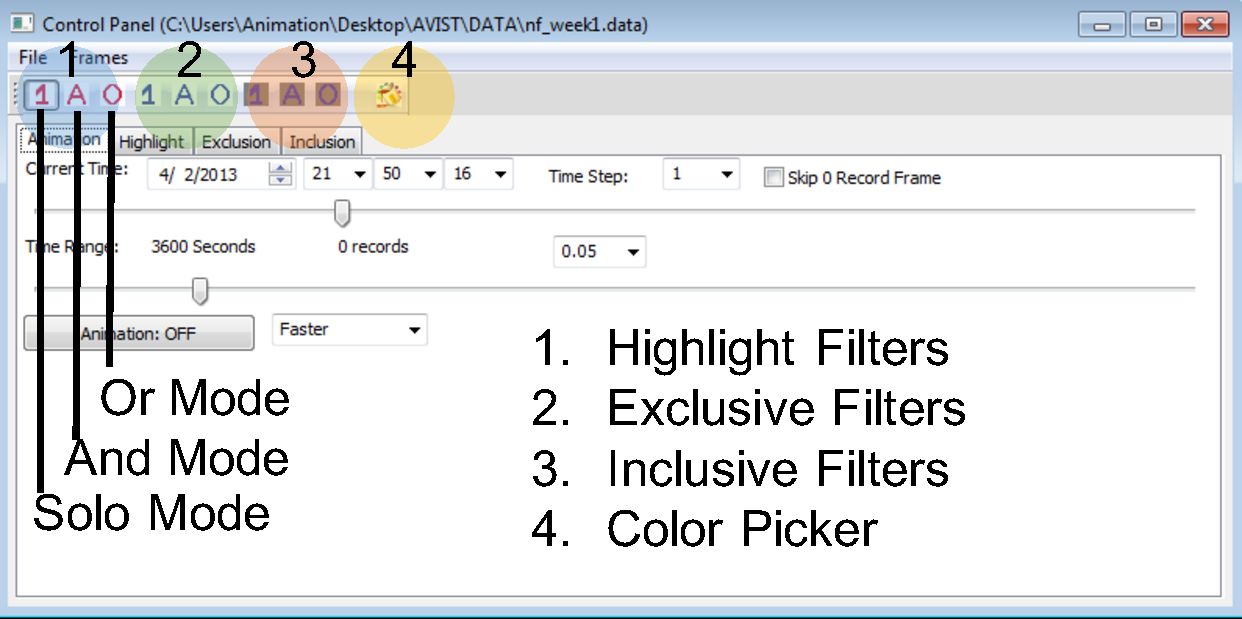
\includegraphics[width=1.0\linewidth]{pic/control.pdf}
	\parbox[t]{1.0\columnwidth}{\relax
	}
	%
	\caption{\label{fig:control} The control panel of AVIST. Three filters (\textit{highlight filter, exclusive filter} and \textit{inclusive filter}) with three modes (\textit{solo} mode, \textit{and} mode, and \textit{or} mode) are provided. }
\end{figure} 

%\begin{itemize}
	\subsubsection{Animation}
	The animation interactions include automatic forward playback, interactively dragging of the time window bar, and interactive change of animation speed. By changing the current time and time range, the time window is customized  to slice data into snapshots, which will be analyzed and visualized at the correlated data views. By combining automated animation with these correlated views, AVIST can provide temporal changes in the datasets, which supports  discovery temporal patterns for further analysis.
	\subsubsection{Filtering}
	Three different filters are implemented in AVIST (their usabilities are shown in following case studies).
	\begin{enumerate}[noitemsep]
		\item \emph{highlight filters}, which make the selected data items stand out of the rest data with different colors.
		\item \emph{exclusive filters}, which remove uninteresting data  items.
		\item \emph{inclusive filters}, the exact opposite of exclusive filters, which remove all data items except those marked by an analyst.
	\end{enumerate}
	Each data filter has three modes: 
	\begin{enumerate}[noitemsep]
		 \item \emph{solo} mode , which allows only one filter item in current filter set.
		 \item \emph{and} mode, which combines several filters together as a whole for emphasizing that data records need satisfy all requirements.
		 \item \emph{or} mode, which means that data records just need to meet only one of the filter requirements.
	\end{enumerate}
	 Based on these three basic filters with their three modes, analysts can nest them to generate complex data filters and apply them to different data views,  which help them to drill down each piece of data record to ``find a needle"  on demand. %These filtering interactions are implemented for each data view to support cross filtering, which enables analysts to reveal hidden insights.


	\subsubsection{Capacities}
The animation interactions can slice  high velocity data into fine-grained subsets by narrowing down the size of time windows; filtering interactions can extract relevant records for concentrating small subsets of high volume data. These interactions transform the large data into small size by removing uninteresting items or highlight important ones, which ensures the flexibility of exploring large multidimensional datasets. In all, AVIST highlights animation and cross-filtering for exploring data by considering its big volume and high velocity features.








 
 
 \section{Performance}

We test the performance of AVIST on a desktop computer, running Windows 7 Enterprise, which is equipped with an Intel i7 processor and a NVIDIA GeForce GTX 680 graphics card with 4GB memory. We use the network traffic dataset from case study one as our benchmark.  

\begin{figure}[htb]
	\centering
	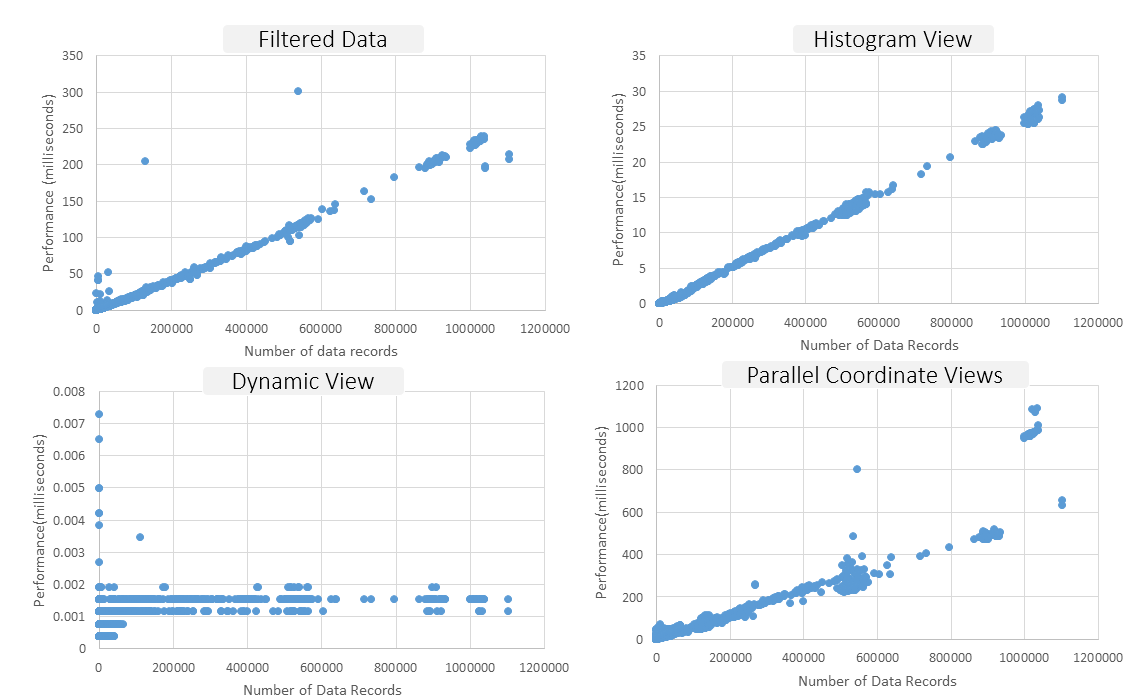
\includegraphics[width=1.0\linewidth]{pic/perf.png}
	\parbox[t]{1.0\columnwidth}{\relax
	}
	%
	\caption{\label{fig:performance}
		The performance of AVIST. The scatter plots show the relationship between number of queried data records and the performance (milliseconds). From the top left to the bottom right are the performances of filtered data, histogram view, time-series view and parallel coordinate views (four axes).  }
\end{figure}

We characterize  AVIST performance in two stages. The first stage is about filtered data generation, which is shared by all data views. The second stage is about each data view visual primitives generation, and their performance are independent with each other. Figure \ref{fig:performance} shows the tested performance in scatter plots. 
It shows a linear relationship between the performance and the queried data records beside time-series view.
Actually, the aggregated information in time-series view can be easily derived by the filtered dataset. The performance of parallel coordinate view is the bottleneck of AVIST. In the plot, we see that if the number of queried records exceeds 600,000, AVIST can not afford real time animation and interaction due to the hardware computation limitation. This also suggests that  users should filter more data in current time window or shrink the time window  for drilling down data details.

\begin{figure}[htb]
	\centering
	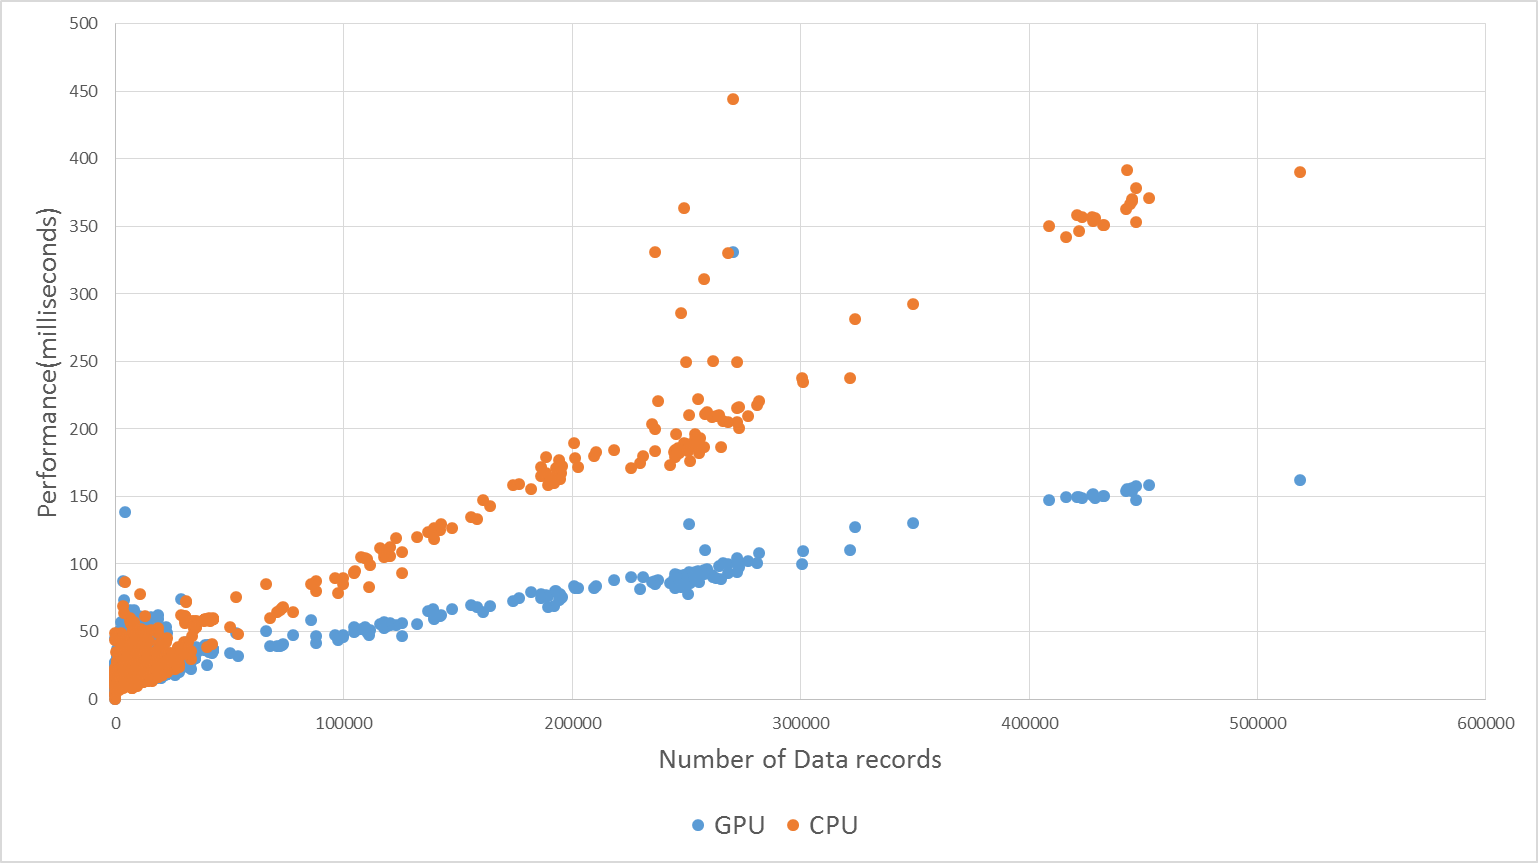
\includegraphics[width=0.75\linewidth]{pic/cmp.png}
	\parbox[t]{1.0\columnwidth}{\relax
	}
	%
	\caption{\label{fig:cmp} The performance comparison between CPU and GPU of parallel coordinate plots (two axes) }
\end{figure}

We also compare the performance between CPU and GPU. Figure~\ref{fig:cmp} shows the comparison of parallel coordinated plots generated by CPU and GPU. We see that the performance of CPU and GPU both follow the linear relationship with the number of data records. However, the performance of GPU is about 2.7 times faster than CPU.

%\section{Related Work}

For visual exploration of big datasets, four questions outline the discussion of related work: 1) which type of data should be visualized, and what is the characteristic; 2) how to store and manage big data; 3) how to compute big data and achieve better performance; 4) how to explore and interact with big data.

\subsection{The Exploration of Multidimensional Datasets}
Large multidimensional datasets are very common and ubiquitous. Most of them are usually behavioral data that are generated by people or machines, which have a natural temporal ordering (streaming data)~\cite{Canny}. Besides the large volume,  high velocity is also an important consideration for analyzing such multidimensional datasets~\cite{IBM2011}. For example, network logs and financial transactions can be generated millions per second. When faced with large volume and high velocity multidimensional datasets, analysts may not know what they are looking for; they will know something is interesting only after they find it. In this setting,  analysts have no idea how to formulate their queries. Thus, the data exploration of large time-series and multidimensional datasets is the key ingredient for knowledge discovery~\cite{harvard}.

The exploration driven system for knowledge discovery becomes a novel requirements in the era of ``Big Data". The data exploration becomes a first class for making sense of large streaming multidimensional datasets. Our paper tackles this problem and provides a solution for building an exploration oriented tool by considering the large volume and high velocity datasets.
%handling big data considering: 1) the volume of data (length of data); 2) the velocity of data (speed of data); 3) the attributes of data (width of data). 

\subsection{Big Data Management}
The data management methods vary based on the size of datasets. If a dataset can fit into the computer memory,  the data layout methods and data structure design should be investigated. When a dataset size is larger than the computer memory capacity, data prefetching and out-of-core techniques need considered~\cite{OFC}. If a dataset is even bigger than the computer disk capacity, the distributed file systems such as HDFS (Hadoop Distributed File System)~\cite{HDFS} can be a choice. 

This paper aims to achieve real-time performance for visual exploration of big data on a commodity desktop. Thus it only considers that datasets can fit into the computer memory. Previous researches, such as  imMens~\cite{2013-immens}, use one million or more data items as a threshold. Thus, this paper follows this definition and gives an upper bound of  big data: the capacity of the computer memory.

To manage big data, especially the multidimensional (tabular) datasets, on computer memory, there are two general ways: row oriented format and column oriented format. Abadi et al.~\cite{Abadi:2008} discussed the differences between these two methods, and pointed out that column format can apply compression techniques to significantly reduce data size and improve query performance. For example, Tableau's TDE is based on column oriented format for managing big data.

Data modeling, sampling and aggregation~\cite{2013-immens} are other ways for handling big data. These methods reduce big data into small size based on data precomputations. However, these kinds of  visual explorations are constrained by precomputation methods, and cannot afford flexibility and low level data details. Our paper emphasizes  visual exploration data fine-grained details by complex filtering and highlighting. Thus, we manage the big multidimensional datasets in row oriented format, and utilizes parallel computing for visual exploration of big data on demand. %Section 3 gives more discussion about it.

\subsection{The GPU Acceleration}

Contrasted with CPUs, graphics processing units (GPUs) have two unique features.

\begin{itemize}
	\item More cores and fine levels of parallelism. GPUs are many-core architecture, which may have thousands of cores.  This feature makes the GPUs  specialized compute-intensive, highly parallel computation. 
	\item Higher memory bandwidths. This means that  GPUs can access data in a fast way (usually more than 100GB/s), or more data in a fixed time period.
	%	\item Weak data cache and flow control. GPUs lack of complexity cache organization and sophisticated branch predication.
\end{itemize}

GPUs are more popular in scientific computing and visualization~\cite{volume}, and several factors have hampered them as general-purpose computing in information visualization and visual analysis fields. Primarily GPUs lack of complexity cache organizations and sophisticated branch predications, which makes the complicated sequential algorithms hard to be parallelized on the GPU platform. In fact,  the development of GPU libraries (e.g., Thrust and cuBLAS) lowers the bar for transforming these algorithms to the GPU platform. Another consideration is slow transfers from CPU to GPU memory, and the limited GPU memory size. However, transfer speeds have improved significantly thanks to PCI-bus improvement, and now the GPU memory capacity is quite good (the latest Nvidia Geforce GTX TITAN Z has 12GB memory).  All these GPU developments make it as a possible solution for handling big data to support exploratory data analysis~\cite{Pawliczek}. 

In fact, GPUs have a deep root in graphics and visualization, and they are good at handling million of pixels. This paper aims to utilize GPUs' fine computing parallelism and high memory bandwidths to support exploratory visual analysis of large multidimensional datasets. Thus, we propose AVIST, which is an animated visualization tool, implemented based on a GPU-centric design for visually exploring big time-series and multidimensional datasets. 

\subsection{Big Data Exploration}
Querying is one of the fundamental interaction techniques for exploring data. Polaris~\cite{polaris} features a visual querying language by integrating analysis and visualization of multidimensional datasets. Analysts can construct sophisticated visualizations by simple drag-and-drop operations. However, Polaris is incapable of managing big data. Tableau, the successor of Polaris, makes a big progress for the big data visualization.  whereas it lacks flexible visual filtering for investigating data details.

Animation is a kind of time multiplexing technique~\cite{Fekete} for visualizing large data items. Moreover, it can effectively reveal temporal patterns by significantly improving graphical perception~\cite{animated}. This paper highlights animation interactions for slicing big data into details. Cross-filtering~\cite{weaver2010} is a method for flexible visually drilling-down into fine-grained relationships for multidimensional datasets. Hence we emphasize cross-filtering and utilize the GPUs to improve performance, to achieve fast, flexible and detailed data exploration. 



      
%\section{Design Analysis}
We emphasize interactively visual exploration of large time-series and multidimensional datasets. 
We believe that big data VA systems need to support analysts \textsl{finding a needle in haystack}, which means that VA systems should provide \textsl{dynamic querying and drill down filtering} functions to help analysts find outliers and identify pattens. 
Based these goals, we summarize  related techniques and present their tradeoff analysis. 

\subsection{Data Processing}
%First, we focus on data processing. We want to achieve both high performance and support for ad hoc querying in our VA system.  
Data processing is important for efficiently organizing data to support interactive exploratory analysis. Based on the survey, we summarize four techniques which are widely used to handle big data.

1) \textbf{In-memory database} is a popular technique in commercial big data VA products. 
Compared with traditional on-disk databases, in-memory databases are faster at accessing data by eliminating disk seeking time
%, which guarantees faster and more predictable performance. 
While the memory capability constrains  data size, solutions, such as hybrid database systems or distributed in-memory architectures~\cite{Kallman:2008},  are directions for future research.  

2) \textbf{Data cube}~\cite{gray} is an aggregation operator for On-Line Analytical Processing (OLAP) in the context of data warehousing. 
However, cube size explodes as data dimensionality increases, which has a significant storage requirement than original datasets. 
Moreover, data cube needs heavily pre-computing for aggregation and hardly support  querying down to individual record.

3) \textbf{Approximated and incremental queries} are promising techniques for big data analysis. 
Fisher et al.~\cite{FisherCHI2012} show the utility of the approximated queries by interviewing three teams of analysts.
They conclude that incremental query for data analysis is tractable and desirable, analysts can obtain immediate feedback by incremental queries to refine their results, even further to explore new avenues.  

4) \textbf{Data reduction} refers to methods for reducing big data with small data, which includes filtering, sampling, aggregation and modeling. 
Liu et al.~\cite{2013-immens} survey data reduction techniques and summarize that both sampling strategies and model based abstractions require prior knowledge and preprocessing of big data. They argue that filtering and aggregation techniques are more effective in some cases, so they choose data cube based aggregation to support  visual query of big data. However, imMens is constrained by per-aggregated data, which cannot support dynamic  filtering. 


\begin{table}[ht]
	\small
	\caption{Database Design Analysis}
	\begin{center}
		\begin{tabular}{|cc|c|c|}
			\hline
			\multicolumn{2}{|c|}{\textbf{Technique}} & \textbf{Pros} & \textbf{Cons} \\
			\hline
			\multicolumn{2}{|c|}{In-memory database} & Fast performance & Memory size limitation\\
			\hline
			
			\multicolumn{2}{|c|}{	\multirow{3}{*}{Data cube} }& Fast performance  & Dimension scalability\\
			& & Aggregation query  & Lack of drill down query \\
			& & & pre-computing\\
			\hline
			
			
			
			\multicolumn{2}{|c|}{Incremental Query} & Fast performance & Approximated query\\
			\hline
			
			
			\multicolumn{1}{|c|}{\multirow{5}{*}{Data Reduction}}& Sampling & Fast performance  & Prior-knowledge\\ 
			& \multicolumn{1}{|c|}{Modeling}  & reduction & pre-computing \\  
			\cline{2-4}
			& \multicolumn{1}{|c|}{Filtering} & dynamic query & in-place computing\\ 
			\cline{2-4}
			& \multicolumn{1}{|c|}{\multirow{2}{*}{Aggregation}} & Fast performance & Lack of drill down query\\
			& \multicolumn{1}{|c|}{} & reduction  & pre-computing\\
			\hline
			
			
			\hline
		\end{tabular}
	\end{center}
	\label{tab:database}
\end{table}



Table~\ref{tab:database} shows a summary of these techniques.
We believe that none of them can be ``one size fits all". Several techniques should be combined together to design a VA system. In AVIST, we store raw data in GPU memory (\textit{in-memory database}), use a data dependency graph for depicting data transformations (\textit{aggregation}) based on users' demands (\textit{dynamic queries}).
%we are inspired by in-memory database, incremental query, filtering and aggregation. 

%Table~\ref{tab:database} present  summaries of these techniques, which are the guides for designing VA systems. Actually no one  is ``one size fits all", several techniques should be combined together in a VA system. In AVIST system, we use in-memory database, incremental query, filtering and aggregation for analyzing big data. 
%Our paper aims to support dynamic querying and drill down filtering, data cube is not our choice. 
%Data sampling and modeling techniques need prior knowledge of the data, which are out of our options. 
%So we choose the in-memory database, incremental queries, filtering and aggregation methods for designing VA system. 






\subsection{Visualization and Interaction}
%Second, we explore existing big data visualization and interaction techniques. Especially, we focus on visualization and  interaction of large high dimensional datasets.


\subsubsection{Visualization}
%The visualization techniques are very important for exploratory analysis system. 
%We summarize major visualization techniques especially considering multidimensional data, which are listed as follows:
We analyze three visualization techniques for exploratory analysis of time-series and multidimensional datasets for designing one view, multiple views and relationships between different views.

1) \textbf{Parallel coordinate plots (PCPs)}~\cite{Inselberg} are a widely used technique for visual analysis  multidimensional data in one view,  which maps each point as a polyline among the parallel axes. 
It scales very well with the number of data dimensions. 
However, it may turn into visual clutters with the rapid growth in the size of datasets. Another consideration is the ordering of axes, which may impact the visual results.



2) \textbf{Scatterplot matrix (SPLOM)}~\cite{ Elmqvist2008g} is a well-established technique to visually explore multidimensional datasets.
It arranges scatter plots of all possible dimension combinations to visualize different aspects of datasets. 
Thus, the number of scatter plots quadratically grows with  data dimensions and the drawing area becomes smaller. 
Over-plotting may happen by increasing the number of points, so analysts may be difficult to make decisions due to visual clutter. 

3) \textbf{Coordinated and multiple views (CMVs)}~\cite{ Roberts} are widely used for exploratory analysis. 
They allow users to see  data in various forms, manipulate the visual presentation in different ways,  and interact and coordinate interactions between multiple views.  
Multidimensional datasets include different data types, which may need various visual presentations. Thus, CMVs are a appropriate design for visualizing multidimensional datasets.



AVIST is built based on coordinate and multiple views. It currently includes histogram view (\textit{aggregation information}), dynamic view (\textit{history information}) and parallel coordinate plots (\textit{detailed information}). More data views can be flexibly added by incorporating the data dependency graph design. 
%While we admit that we may not list all possible visualization techniques for multidimensional data, these three are the most important methods. In our VA system design,  we favor coordinated and multiple views, and parallel coordinate plots instead of scatterplot matrix. 

\subsubsection{Interaction}
AVIST highlights visual filtering and querying. Three interaction techniques are considered targeting large time-series and multidimensional datasets.

 
%User can control the visual items by animation and interaction techniques. We list three common animation and interaction techniques for exploratory data analysis.

1) \textbf{Brushing and linking} (\textit{multidimensional feature}) is used to explore tightly coupled data relationships by highlighting items in multiple views. 
%imMens~\cite{2013-immens} is an example to highlight brushing and linking technique for visual querying big data. 
Cross-filtering~\cite{weaver2010cross} generalizes the brushing and linking technique into a design pattern for fast and flexible  drilling down into fine grained relationships in multidimensional datasets. In AVIST, we couple brushing and linking with coordinate and multiple views. A data dependency graph is inspired by cross-filtering pattern for charactering the data flow.


2) \textbf{Animation} (\textit{time-series feature}) is viewed as special filter based on time. 
It automatically updates data items between time frames. During the frame transitions, temporal patterns can be revealed. 
Compared with brushing and linking, which can be regarded as a space multiplexing technique, animation is a kind of  time multiplexing technique for visualizing data items at a regular pace.  AVIST  emphasizes animation for slicing data from time domain to reduce computation overhead. In addition, animation is also a good way for revealing temporal  patterns and trace history behaviors. 

3) \textbf{Dynamic query} (\textit{big data feature}) means interactively filtering and displaying of the data items through successive interactions. Brushing and linking as well as animation as ``range-silder" are  general methods for dynamic queries. To explore the multidimensional datasets, more complex filters and queries need be investigated. We design and implement combined data filters in AVIST to support complex querying. Three different filters (\textit{highlight filters, exclusive filters and negative exclusive filters}) and three filter modes (\textit{solo mode, and mode, or mode}) can combine together to support complex set algebra for dynamic querying. More details about them are discussed in system design section.
%Zhao et al.~\cite{zhao2013interactive} present a visual query language in PivotSlice to identify implicit and explicit relationship. Polaris \cite{stolte2002polaris} allows users to drag and drop visualizations based on its table algebra.

%Other interaction techniques may also be effective for big data visualization. We believe that the listed three are crucial for exploring big data. We want to incorporate these techniques in our VA system to achieve dynamic querying to help users drilling down each record.


\subsection{Parallel Computing}

Based on our review of parallel computing techniques for VA systems, we choose GPUs to parallelize data processing, rather than distributed system. The reasons of this as as follows.

Firstly, previous MapReduce based systems are designed for long batch jobs instead of small dynamic queries~\cite{Dean:2008}. Spark~\cite{Zaharia:2010} presents resilient distributed datasets  for reusing a previous working set  of data based on MapReduce, which boosts the performance of interactive analysis applications. However, a key concept of MapReduce based systems is shipping the computation to a cluster of nodes, ignoring large data shipping between nodes.  We argue that visual analysis of big data needs shipping large visual primitives data from different nodes into GPU memory. This IO cost may become a bottleneck of VA systems. Compared with distributed systems, AVIST highlights GPU parallel processing and rendering simultaneously. This kind of design avoids 1) data shipping between nodes and 2) data communications between GPU memory and main memory.  However, AVIST is limited by current GPU memory capability. We acknowledges this, and believe that AVIST can handle more with GPU technology increases. 
%Our paper demonstrate that  AVIST system as a proof of concept shows that GPU based big data visual analysis is a feasible solution.     
%This section gives a brief trade-off discussions of parallel platforms for designing a VA system. 

%\textbf{Distributed systems} are becoming a hot topic for big data visual analysis, and many distributed VA systems have already deployed, such as Google's Dremel~\cite{melnik2010dremel}. However most of them are based on Map-Reduce scheme~\cite{Dean2008}, that they are designed for large, long-running bath jobs  and are incapable of many small, short and increasing interactive queries~\cite{Chen:2012}. To make best use of distributed systems, Dremel~\cite{melnik2010dremel} contributes a novel data model, which is a columnar representation of nested data for dynamic query. Moreover, Starfish~\cite{herodotou} characterizes the work load of distributed systems and applies optimization for scheduling jobs to achieve better performance. However, such kinds of improvements focus on shipping the computation to a cluster of processing nodes, while shipping large data in the cluster increases I/O costs, which may not achieve real time performance for interaction with big data. 

%Such systems for visual analysis big data are mainly based on data aggregation techniques, which needs high computing of big data and small statistical results. When user want to see million items, the network throughput can not afford real time transforming such big data from cloud database into user's screen.      

%\textbf{GPUs} are another potential solution for analyzing big data. Besides their powerful rendering capability, GPUs feature the general purpose computing. 
%For example, Fekete et al.~\cite{Fekete:2002} suggested utilizing GPU rendering power to achieve the redisplay speed required for smooth interaction of big data. When user triggers a series of queries, all data items are send to the GPU for fast rendering.  imMens~\cite{2013-immens} makes a further step for visually querying big data based on GPU parallel computing. However, GPU based solutions suffers limitations, such as limited GPU memory size, copying  data back and forth between CPU and GPU, which increases I/O costs. 

Table~\ref{tech} presents a brief summary of all mentioned techniques we have incorporated into the design  AVIST.   

%Generally, parallel computing is promising for big data VA system and both distributed systems and GPUs are the feasible solutions. In our system design, we leverage the power of GPUs for fast rendering and parallel computing. We acknowledge the shortcomings of GPUs, and try to overcome them to achieve good performance. Table~\ref{tech} shows the summary of all mentioned techniques we try to incorporate into our VA system.   


\begin{table}[h]
	\small
	\caption{Summary of VA system techniques}
	\label{tech}
	\begin{tabular}{|c|c|c|c|}
		\hline
		\textbf{Database}                                                                          & \textbf{Visualization}                                      & \textbf{Interaction}                                                                             & \textbf{GPU}                                                                         \\ \hline
		\begin{tabular}[c]{@{}c@{}}In-memory\\ Incremental Query\\ Filtering \\ Aggregation\end{tabular} & \begin{tabular}[c]{@{}c@{}}PCPs\\ CMVs\end{tabular} & \begin{tabular}[c]{@{}c@{}}Brushing \& Linking\\ Animation\\ Dynamic Query\end{tabular} & \begin{tabular}[c]{@{}c@{}}Fast Rendering\\ GPU Computing\end{tabular} \\ \hline
	\end{tabular}
\end{table}

%In this section, we first emphasis our design principles for exploratory big data visual analysis system, then we analyze the related requirement based on the design principles. //design requirements

%\subsection{Design Principle}
%To support exploratory data analysis, we emphasis the following principles 


%\textbf{P\RN{1}: Finding a needle in haystack } raw data, reduction, sampling , approximated results is useless 



%\textbf{P\RN{2}: Real time visualizating million nodes on desktop compupter} need GPU computing and rendering, latency and data throughput.


%The first challenge for big data visual analysis system is intensive computing scaling to big data size. Previous research proposed different methods, such as data reduction and sampling, approximate database query, incremental computing and parallel processing. While we aim to help users to \textbf{find a needle in haystack} for exploratory data analysis, we adopt the \textbf{incremental computing and parallel processing} ideas, abandoning the data reduction and approximated query methods.

%Another consider issues for designing big data system is the low latency and high throughput of big data.   abstract
%%%here now


%\section{GPU based In-Situ Visualization Architecture}
Wong et al.~\cite{wong2012top} list top 10 challenges of extreme-scale visual analysis, and \emph{in-situ} analysis ranks the top one. Compared with traditional approaches, in situ VA tries to perform as much analysis as possible while the datasets are in memory for reducing I/O cost. In scientific visualization, in-situ processing and visualization are the general methods for handling big data \cite{ma2007situ},  when I/O becomes the performance bottleneck. 
%The idea is that simulation and visualization code run simultaneously which can reduce the data transfer and storage costs. 
In this paper, we adopt \emph{in-situ} concept, and propose that 
\textbf{data processing and visualization code  run together to reduce the number of visual primitives transferring between GPU memory and main memory}. Thus, all code can run on the GPU to fully utilize GPU parallel resources.

\begin{figure}[htb]
	\centering
	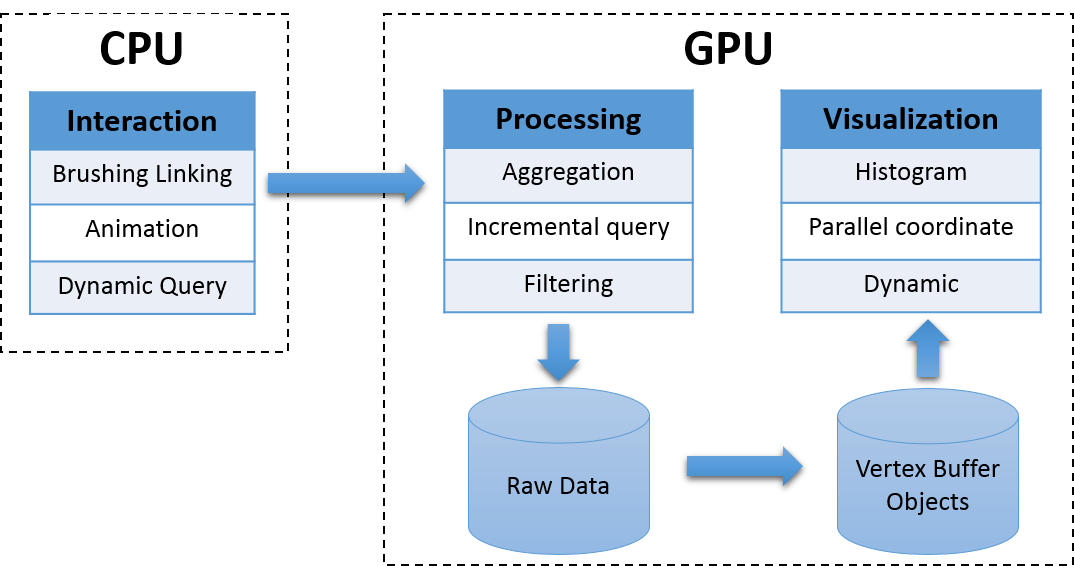
\includegraphics[width=1.0\linewidth]{pic/in-situ.png}
	\parbox[t]{1.0\columnwidth}{\relax
	}
	%
	\caption{\label{fig:architecture} The \emph{In-Situ} visualization architecture of the \emph{AVIST}.}
\end{figure}


Figure~\ref{fig:architecture} shows our GPU based in-situ visualization architecture, which incorporates previous mentioned visualization and interaction techniques. In the CPU sides, it only handles user interactions,  which trigger GPU parallel processing and rendering. The GPU controls all data transformation from  raw data into visualization results. It can process related queries and generate visual primitives simultaneous. All raw data is located in GPU memory to support users' drill-down query of each data record. All generated visual primitives are stored in GPU vertex buffer objects (VBO) to obtain substantial performance gains and avoid data transformation with main memory.
 


Our in-situ visualization architecture makes the best use of GPUs powerful computing and rendering performance. It supports filtering and visualizing items in parallel. More importantly, this kind of design avoids data transformation between main memory and GPU to reduce IO cost, which is potential bottleneck for big data VA systems. 


However, the major consideration of the in-situ visualization architecture is data scalability problem, which is limited by GPU memory capability. To feed more data into the GPU memory, we propose to preprocess datasets into compressed binary format.

%There are also two major considerations in our in-situ visualization architecture. The first one is that data size is limited by GPU memory size, the second is how to deploy incremental computing idea to gain better performance.

%\subsection{Data Preprocessing}
%In our architecture, the data size is limited by GPU memory capability. To feed more data into GPU memory, we preprocess the data into compressed binary format.

Considering general multi-dimensional datasets, we first identify each data type in datasets. For categorical and ordinal data, we count  all possible values and map each value into a unique ID. All values and their corresponding IDs are stored in main memory as meta-data. %While on the GPU memory, we just need to store each value's  corresponding ID. 
Then, we store datasets on GPU memory with their row-oriented format, which replaces the original values to  IDs  in binary format of one byte, two bytes or four bytes (e.g. if one dimension data only has less than 256 possible values, we can use one byte for representation.). For quantitative data, we simply store one \emph{Int} or \emph{Float} for representing each data value. We store  time data in \emph{$time\_t$} format, which occupies 8 bytes. Table \ref{preprocessing} summarizes our data preprocessing strategy. The row-oriented design targets temporal and spatial locality based analytical tasks for drilling-down query, which supports analysts to find  a ``needle in a haystack".  The preprocessing focuses on analyzing each column for compression and making sense of the whole datasets.


\begin{table}[h]
	\centering
	\caption{Data preprocessing methods}
	\label{preprocessing}
	\begin{tabular}{|c|c|c|}
		\hline
		\textbf{DataType}                                                     & \begin{tabular}[c]{@{}c@{}}\textbf{GPU memory}\\ \textbf{binary format}\end{tabular} & \begin{tabular}[c]{@{}c@{}} \textbf{Main memory} \\ \textbf{meta-data}\end{tabular}   \\ \hline
		Time                                                         & \begin{tabular}[c]{@{}c@{}}time\_t\\ 8 bytes\end{tabular}          & \begin{tabular}[c]{@{}c@{}}minimum\\  maximum\end{tabular}         \\ \hline
		Quantitative                                                 & \begin{tabular}[c]{@{}c@{}}Int or Float\\  4 bytes\end{tabular}    & \begin{tabular}[c]{@{}c@{}}minimum \\ maximum\end{tabular}         \\ \hline
		\begin{tabular}[c]{@{}c@{}}Categorial\\ Ordinal\end{tabular} & $1\sim4$ bytes                                                          & \begin{tabular}[c]{@{}c@{}}Dictionary\\ (IDs and data value)\end{tabular} \\ \hline
	\end{tabular}
\end{table}


A standard commercial graphics card has its memory from 4GB to 8GB. Considering a  dataset with most of its data attributes occupy 4 bytes, then the total data items we can handle is about 10 millions. So our VA system can handle million records in one GPU.



%

\section{AVIST}
This section presents the design and implementation of AVIST. The core part of AVIST is a data dependency graph, which incorporated with multiple visualization and interaction techniques for charactering data transformations to highlight data aggregation on demand.  

%Coordinated and multiple views are provided in AVIST. Brushing and linking, animation and dynamic queries are deployed in data views. More importantly, AVIST features a data dependency graph for charactering data transformations, provides data aggregation and visual primitives generations together on demand.
 
\subsection{Visualization and Interaction}

%figure shows the design of the views. parallel 



Three data views are provided: histogram view, parallel coordinated view and dynamic view. More data views can be flexible added. For example, we add a virtual globe view for spatial data visualization in our case studies. Users can directly apply brushing and linking interaction on these views. 

\textbf{Histogram view} shows the data distribution of  current time window. Users can select different dimensions  from a listbox to explore different aggregation information.

\textbf{Parallel coordinate views} show  details of each data record in current window. Users can select multiple data dimensions to generate their custom parallel coordinate plots. The axes can be re-ordered based on users' selected order in the listbox.

\textbf{Dynamic view} is a time series  chart, which shows the data aggregation of certain filtered events over a period of time. When a user change data filters, the dynamic view clears previous results and re-draw everything. 

\textbf{Control panel} provides animation and dynamic query interactions.
%By playing the animation of the data at certain pace,  hidden temporal patterns can be revealed. 
The animation supports automatic forward playback, interactively dragging of the time window bar, and interactive change of animation speed. By changing the current time and time range, users can define a time window in which the information will be analyzed and visualized at the correlated views. By combining automated animation with these correlated views, AVIST provides  temporal changes in the datasets, which supports  discovery temporal patterns for further analysis.

\begin{figure}[htb]
	\centering
	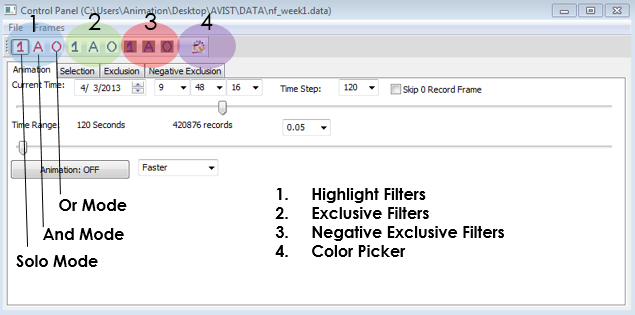
\includegraphics[width=1.0\linewidth]{pic/control.png}
	\parbox[t]{1.0\columnwidth}{\relax
	}
	%
	\caption{\label{fig:control} The control panel of AVIST. Three filters (\textit{highlight filter, exclusive filter and negative exclusive filter}) with three modes (\textit{solo mode, and mode, and or mode}) are provided. }
\end{figure} 

Besides animations, AVIST features the combined data filtering as shown in Figure~\ref{fig:control}. Three different filters are implemented: 1) highlight filters which make users' selected values stand out of the rest data with different colors,  2) exclusive filters to remove non-interesting data from data views and 3) negative exclusive filters, the exact opposite of exclusive filters, which remove all data except items marked interesting by a user. Each kind of data filters have three  modes: 1) \emph{Solo mode} , which allows only one filter value in current filter set, 2) \emph{and mode}  to combine several filters together as a complex filter emphasizing that data records need satisfy all requirements for visualization and 3) \emph{or mode}, which means that data records just need to meet only one of the filter requirements. 
Based on these three basic filters with their three modes, users can nest them to generate complex data filters which help to drill down each piece of data record. These filters with the brushing and linking interaction technique can quickly help users to explore datasets. 
%In Figure~\ref{fig:views}, users choose  highlight filters with \emph{or mode}, and then brush their selected colors in \textit{firstSeenDespIp} axis of parallel coordinated view to identify three suspicious IP addresses. The histogram view shows the distributions of \textit{ipLayerProtocol}, which emphasizes the highlighted activities in TCP flows. The dynamic view shows the highlighted records are a  periodically behavior in the network.

%for visual analysis large cyber security datasets, users can directly apply exclusive filter on port 80 to remove related network records to clear the visualization. After it, all three data views are immediately updated, and potential visual patterns may appear.


\subsection{Data Dependency Graph}

We character data transformations using a data dependency graph, which emphasizes data computation and visualization are on demand, triggered by user interactions. 

\begin{figure}[htb]
	\centering
	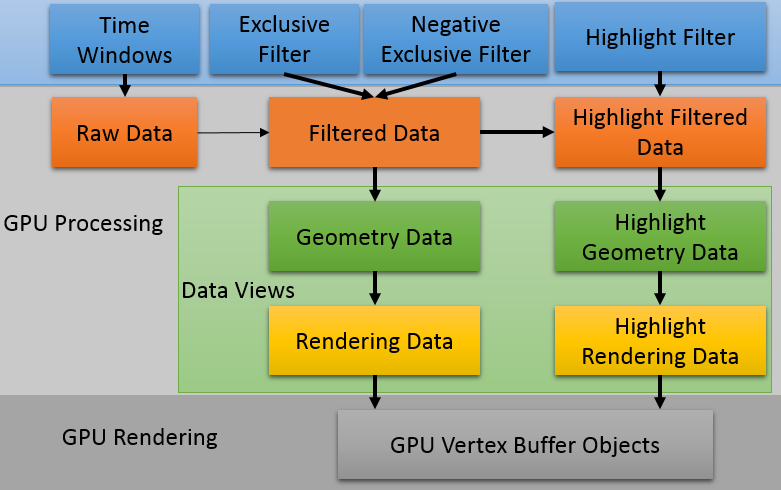
\includegraphics[width=1.0\linewidth]{pic/graph.png}
	\parbox[t]{1.0\columnwidth}{\relax
	}
	%
	\caption{\label{fig:datagraph} The data dependency graph of AVIST, which includes three layers: data filters, data processing and data rendering.}
\end{figure} 

% consider the cross filter design pattern 
%We employ the cross filtering design pattern \cite{weaver2010cross} in our GPU based in-situ visualization architecture, which contributes  a data dependency graph for organizing the data flow on the GPU.

Figure~\ref{fig:datagraph} shows our data dependency graph, which is separated into three parts. Firstly, the top level graph shows the user interactions in CPU side. Users can manipulate four filters generated by their interactions: \emph{time windows}, \emph{exclusive filter}, \emph{negative exclusive filter} and \emph{highlight filter}. All filters are passed into GPU  for data processing. The middle part of the graph is the GPU parallel processing. The raw data is filtered by \emph{time windows} first, then both \emph{exclusive filter} and \emph{negative exclusive filter} are applied to remove relevant data items. At last, \emph{highlight filter} is deployed to generate highlight datasets. Then, there are two steps to transform filtered data into visual primitives of each data view: 1) the geometry data is the aggregation of filtered data; 2) then rendering data follows, which transforms the aggregation data into visual primitives. At last, all rendering data are passed into GPU vertex buffer objects (VBOs). This kind of design makes that all data views share the raw data, filtered data and highlight filtered data, while each data view has its own geometry and rendering data. The last part in this graph is GPU rendering, which transforms all visual primitives into pixel colors.  




Our data dependency graph has several advantages. First, it follows the cross filtering design pattern~\cite{weaver2010cross} and three filters with three modes supports the drill down query of multi-dimensional datasets. 
%Users interactions trigger the data flows to update the visualizations. 
Second, all data processing and visual rendering can fully utilize GPU resources to achieve best performance with minimum IO costs. 
Third,  incremental computing can be applied to exploit temporal and spatial locality. When users play animation, frame-to-frame coherence can be exploited. In such cases, only incremental data need to be considered. Besides, user interactions also follow incremental format for dill-down queries. If a user perform \emph{or} operator of highlight filters, previous highlighting visual primitives do not need to be recomputed. When performing \emph{and} operator, incremental computing is only applied in previous highlight data which trigger the right column of data graph, while all other data are still the same. In all, we formalize the computation flow as a direct acyclic graph (DAG) of tasks, fully incorporated user interactions and incremental computing.

%one page
%// and or not similar with SQL  ad hoc visual query
%//multiple coordinate views space 
%//animation 	time

 
\subsection{Implementation}
AVIST is written in C++, its computation codes are based on CUDA 5.5 and visualization codes are based on OpenGL and GLSL. The interface are coded by wxWidgets. We use the Thrust library\footnote{https://developer.nvidia.com/Thrust} for accelerating sort, scan, transform and reduction operations.


\begin{figure}[htb]
	\centering
	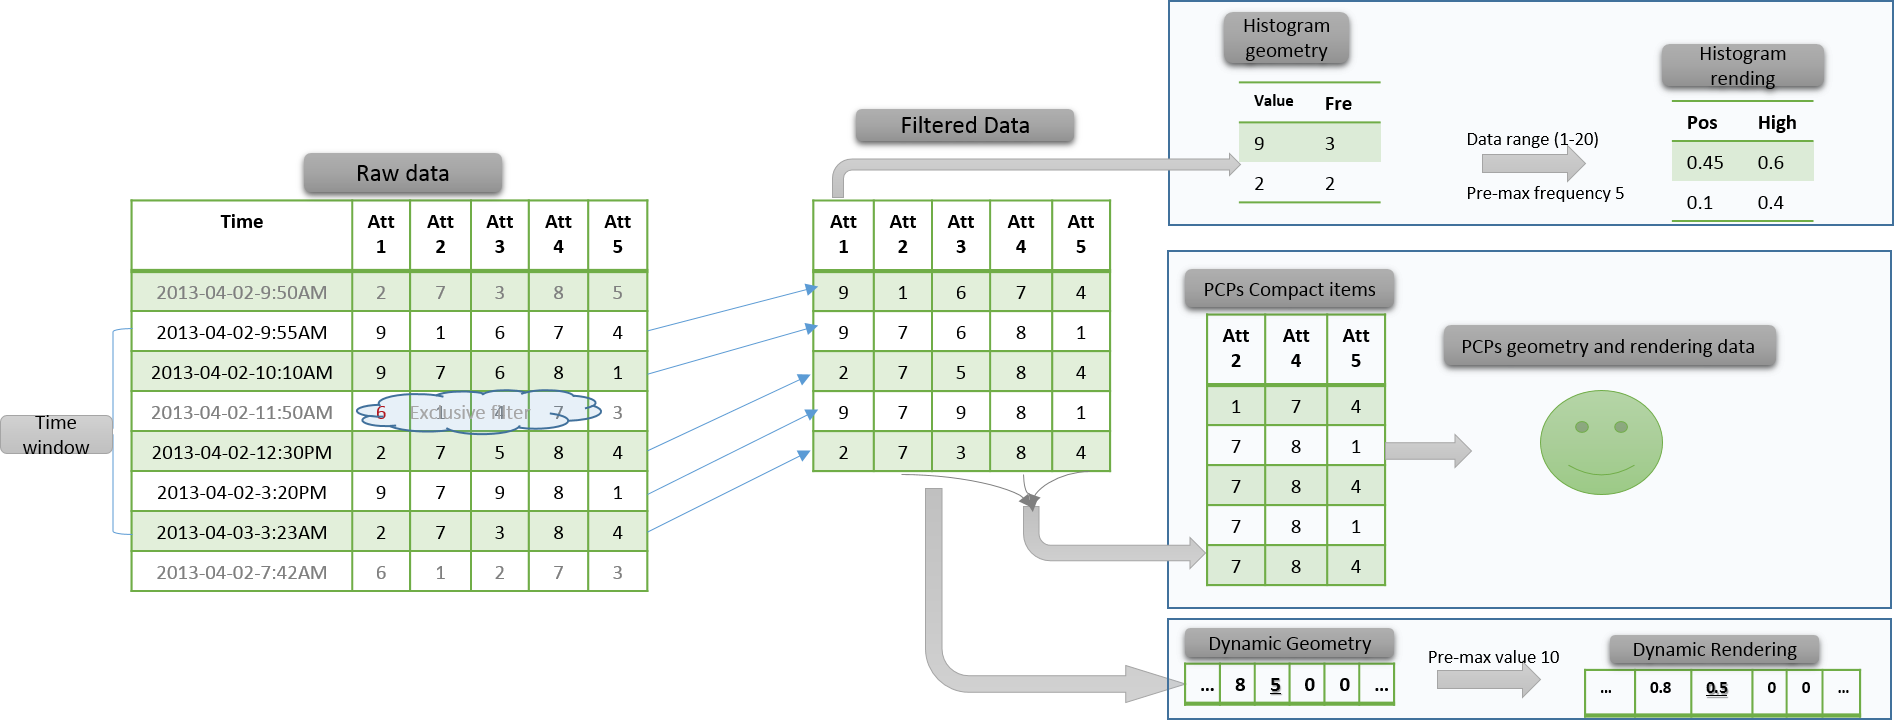
\includegraphics[width=1.0\linewidth]{pic/dataTran1.png}
	\parbox[t]{1.0\columnwidth}{\relax
	}
	%
	\caption{\label{fig:dataTran1} This figure shows data transformations from raw data to  geometry and rendering data of histogram and dynamic view.}
\end{figure} 

\begin{figure}[htb]
	\centering
	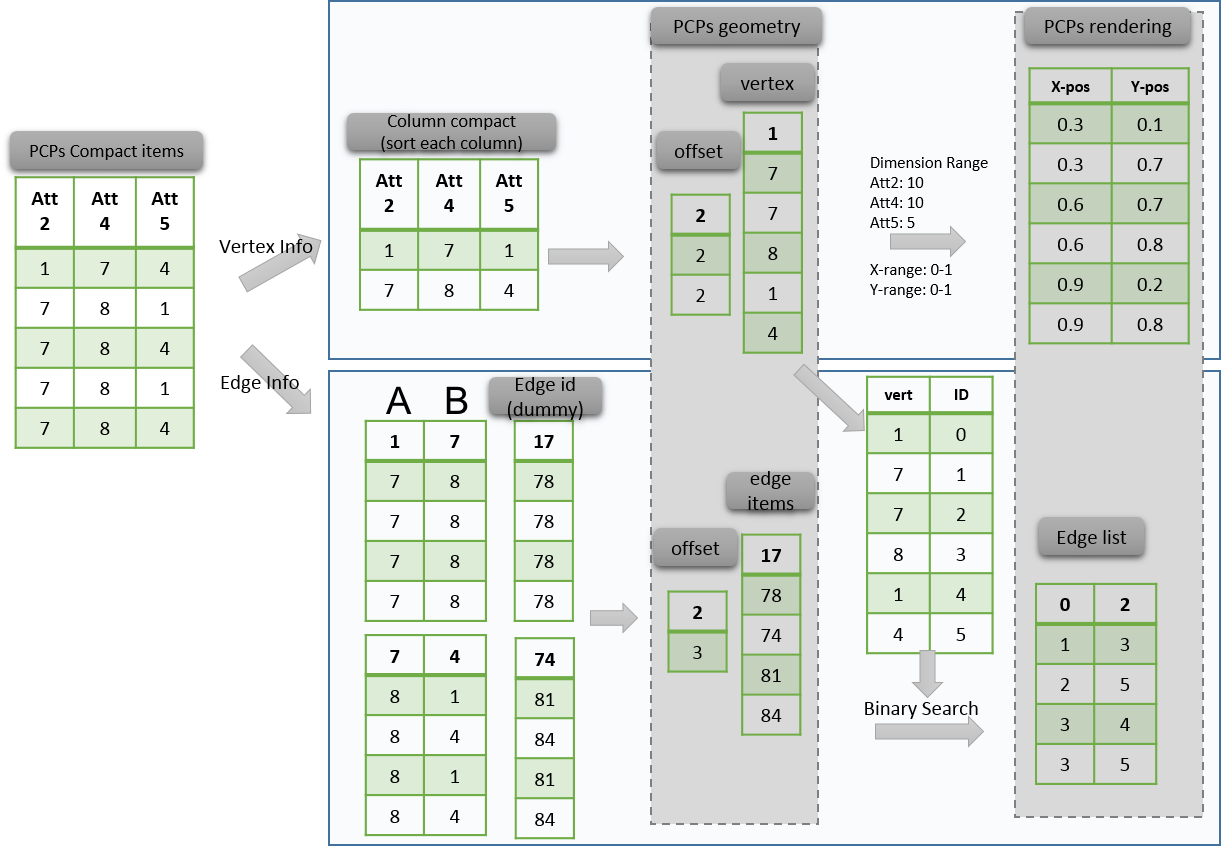
\includegraphics[width=1.0\linewidth]{pic/dataTran2.png}
	\parbox[t]{1.0\columnwidth}{\relax
	}
	%
	\caption{\label{fig:dataTran2} This figure shows data transformations from compact item lists to rendering data in parallel coordinate views. The data transformations are separated into two parts: vertex and edge data generation.}
\end{figure} 

Figure~\ref{fig:dataTran1} demonstrates data transformation from raw data into visual primitives of histogram and dynamic views. Firstly, the time window filter is applied to slice the raw data into current chunk of data. Secondly, each data record in current frame is validated by exclusive and negative exclusive filters in parallel, then they are compacted into a filtered dataset. Based on user's chosen dimension in histogram view, we group the corresponding column data to generate geometry data and transform it to rendering data based on the meta-data (data range). The data of dynamic view is straightforward. GPUs summarize the filtered data items as geometry data, then transform it to height value based on previous maximum value.

Data transformations in parallel coordinate views are more complex than other views. Firstly, GPUs generate PCPs compact items based on user chosen axes. Then the data flow is separated into two branches for generating vertex and edge data. To generate vertexes information, \textsl{unique} operator is applied to each column and then all unique values are organized into \textit{vertex} array and \textit{offset} array. Then the data ranges are applied to geometry data to obtain each node's position.
For edges, every two neighboring columns are combined into an array by their dummy values, then they are compacted and organized into \textit{edge} array and \textit{offset} array.  After this, the dummy values are unpacked, which are separated into two columns for representing edge list. At last, we replace  each vertex ID with its order ID in edge list as the rendering data.  


%\subsection{Filtering on the GPU}
%The implementation of time windows filter is straightforward, and we apply binary search of the raw data to obtain the start and end records within the time window (The raw data is stored chronologically). We generate a boolean vector, and examine each records by the exclusive filter and negative exclusive filter. Then we compact the boolean vector and 
%\subsection{Data View on the GPU}
%The dynamic view and histogram view is simple, and we focus on the parallel coordinate generation on the GPU.
%The input data is the filtered or highlighted filtered data, and the output is the edge list and node position.
%We use shader to generate the stack view and quad.

\begin{figure}[htb]
	\centering
	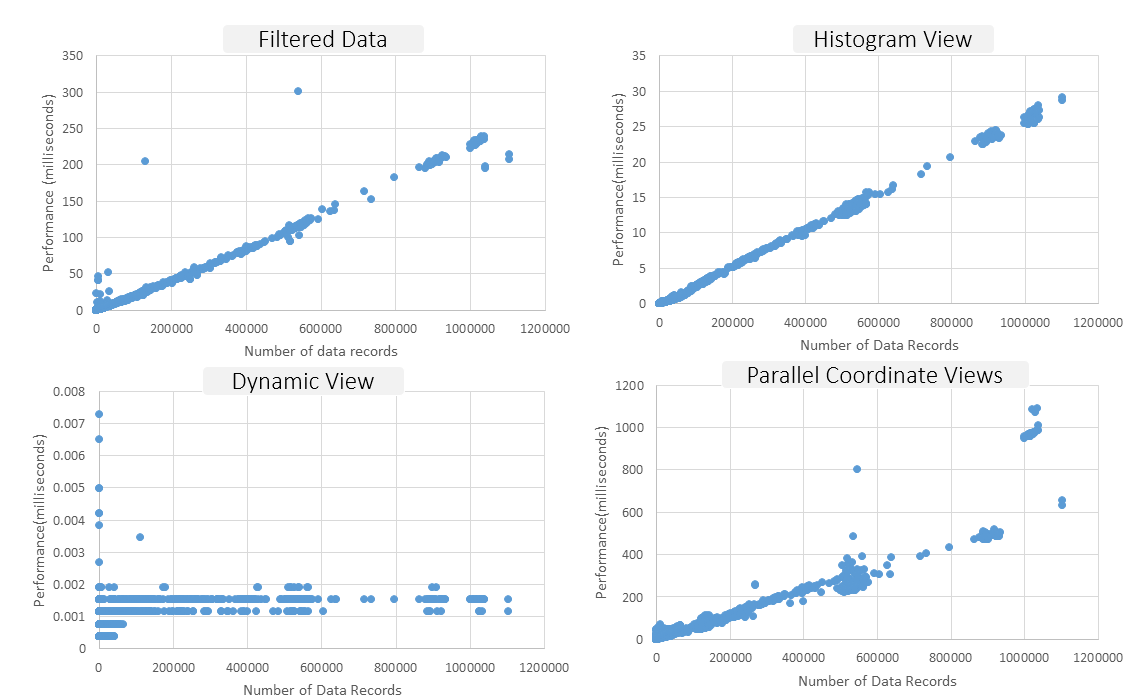
\includegraphics[width=1.0\linewidth]{pic/perf.png}
	\parbox[t]{1.0\columnwidth}{\relax
	}
	%
	\caption{\label{fig:performance}
		The performance of AVIST (without incremental computing). The scatter plots show the relationship between number of queried data records and the performance (milliseconds). From the top left to the bottom right are the performances of filtered data, histogram view, dynamic view and parallel coordinate views (four axes).  }
\end{figure}


\begin{figure*}[htb]
	\centering
	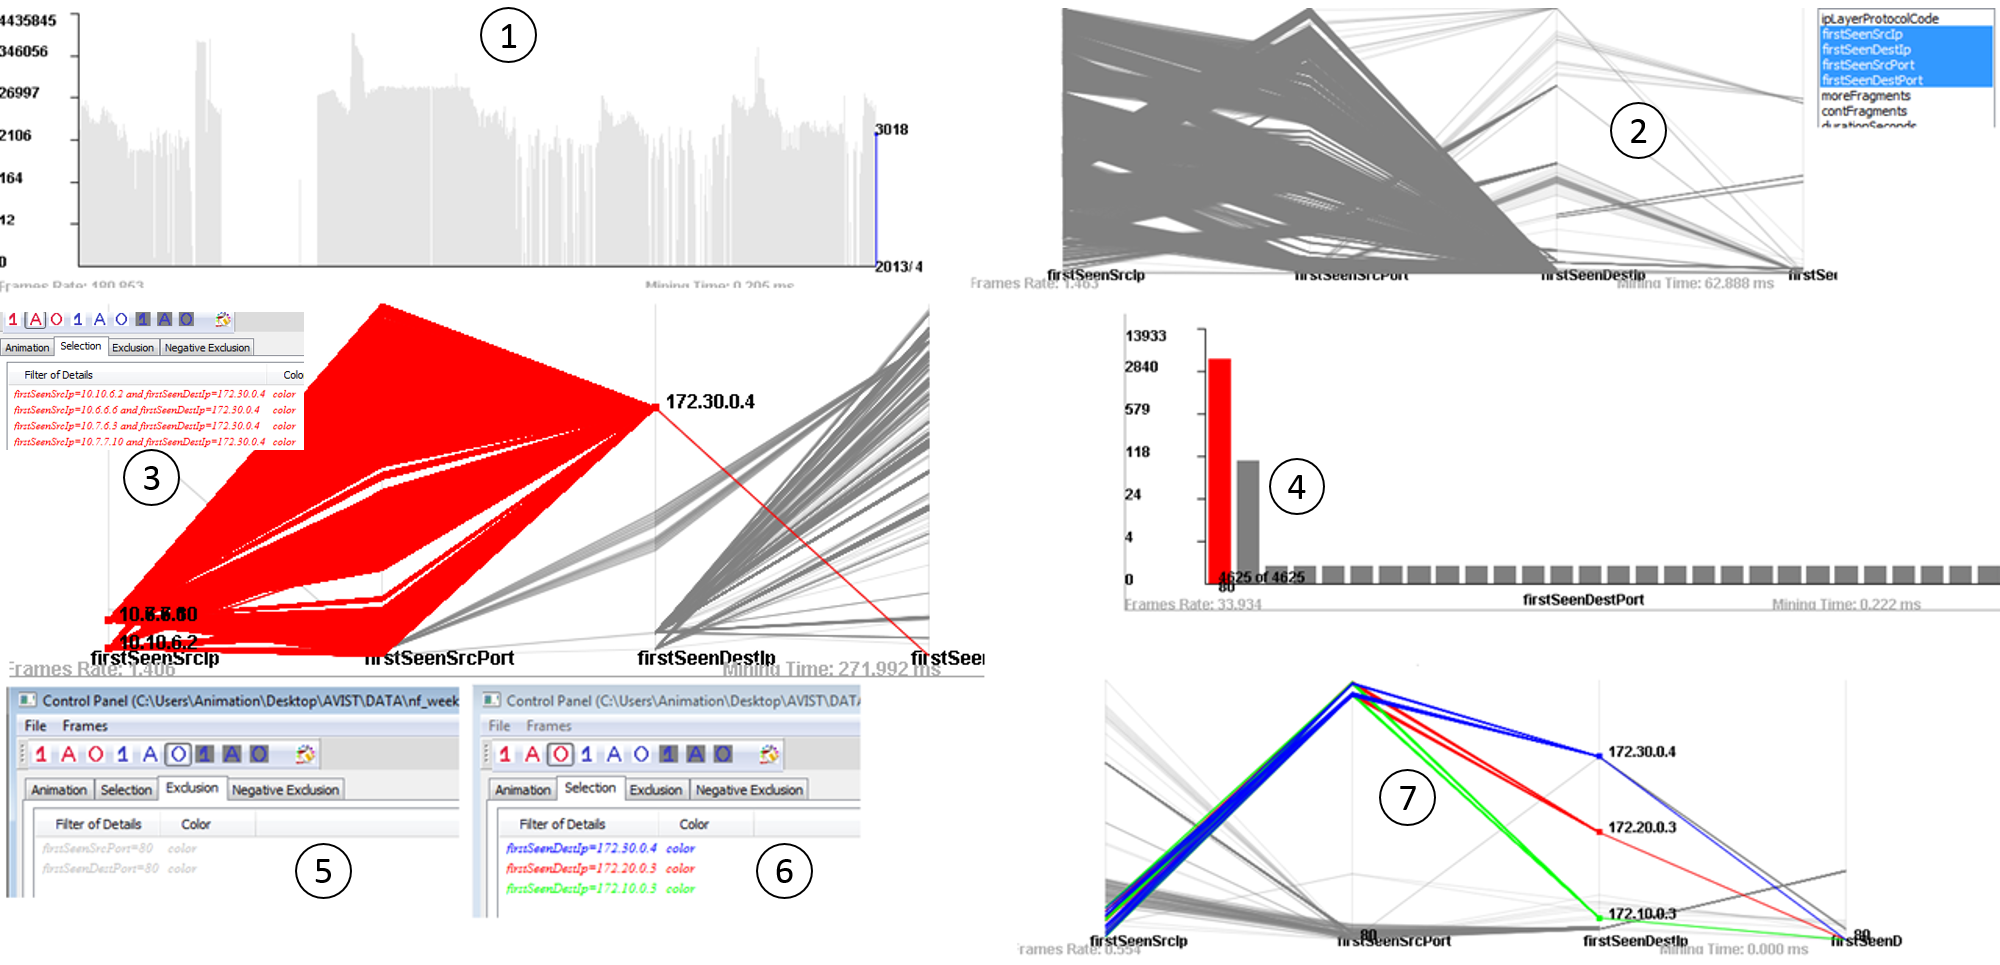
\includegraphics[width=0.9\linewidth]{pic/network2.png}
	\parbox[t]{1.0\columnwidth}{\relax
	}
	%
	\caption{\label{fig:vast}
		This figure shows a usage scenario how AVIST helps analysts to visual explore the large network logs. 
		Seven steps are presented in this figure, and Section 6.1 gives more detailed discussions for each step. }
\end{figure*}

\subsection{Performance}
%The AVIST system is written in C++ and CUDA 5.5. The visualization codes are based on OpenGL and GLSL. The interface controls are coded using wxWidgets.

We test the performance of AVIST on a desktop computer, running Windows 7 Enterprise with Service Pack 1, which is equipped with an Intel i7 processor and an NVIDIA GeForce GTX 680 graphics card with 4GB memory. We use the network traffic dataset from case study one as the benchmark.  



Based on the dependency graph design, we character  AVIST from two stages. The first stage is about filtered data generation. This stage is shared by all data views. The second stage is about each data view visual primitives generation, and their performance are independent with each other. Figure \ref{fig:performance} shows the performance in scatter plots. 
We see there is a linear relationship between the performance and the queried data records beside dynamic view.
Actually, the aggregated information in dynamic view can be easily derived by filtered dataset. The performance of parallel coordinate view is the bottleneck of AVIST. In the plot, we see that if the number of queried records exceeds 600,000, AVIST can not afford real time animation and interaction due to the hardware computation limitation. This also suggests that a user should filter more data in current time window or shrink the time window  for drilling down data details.







%\begin{figure*}[htb]
%	\centering
%	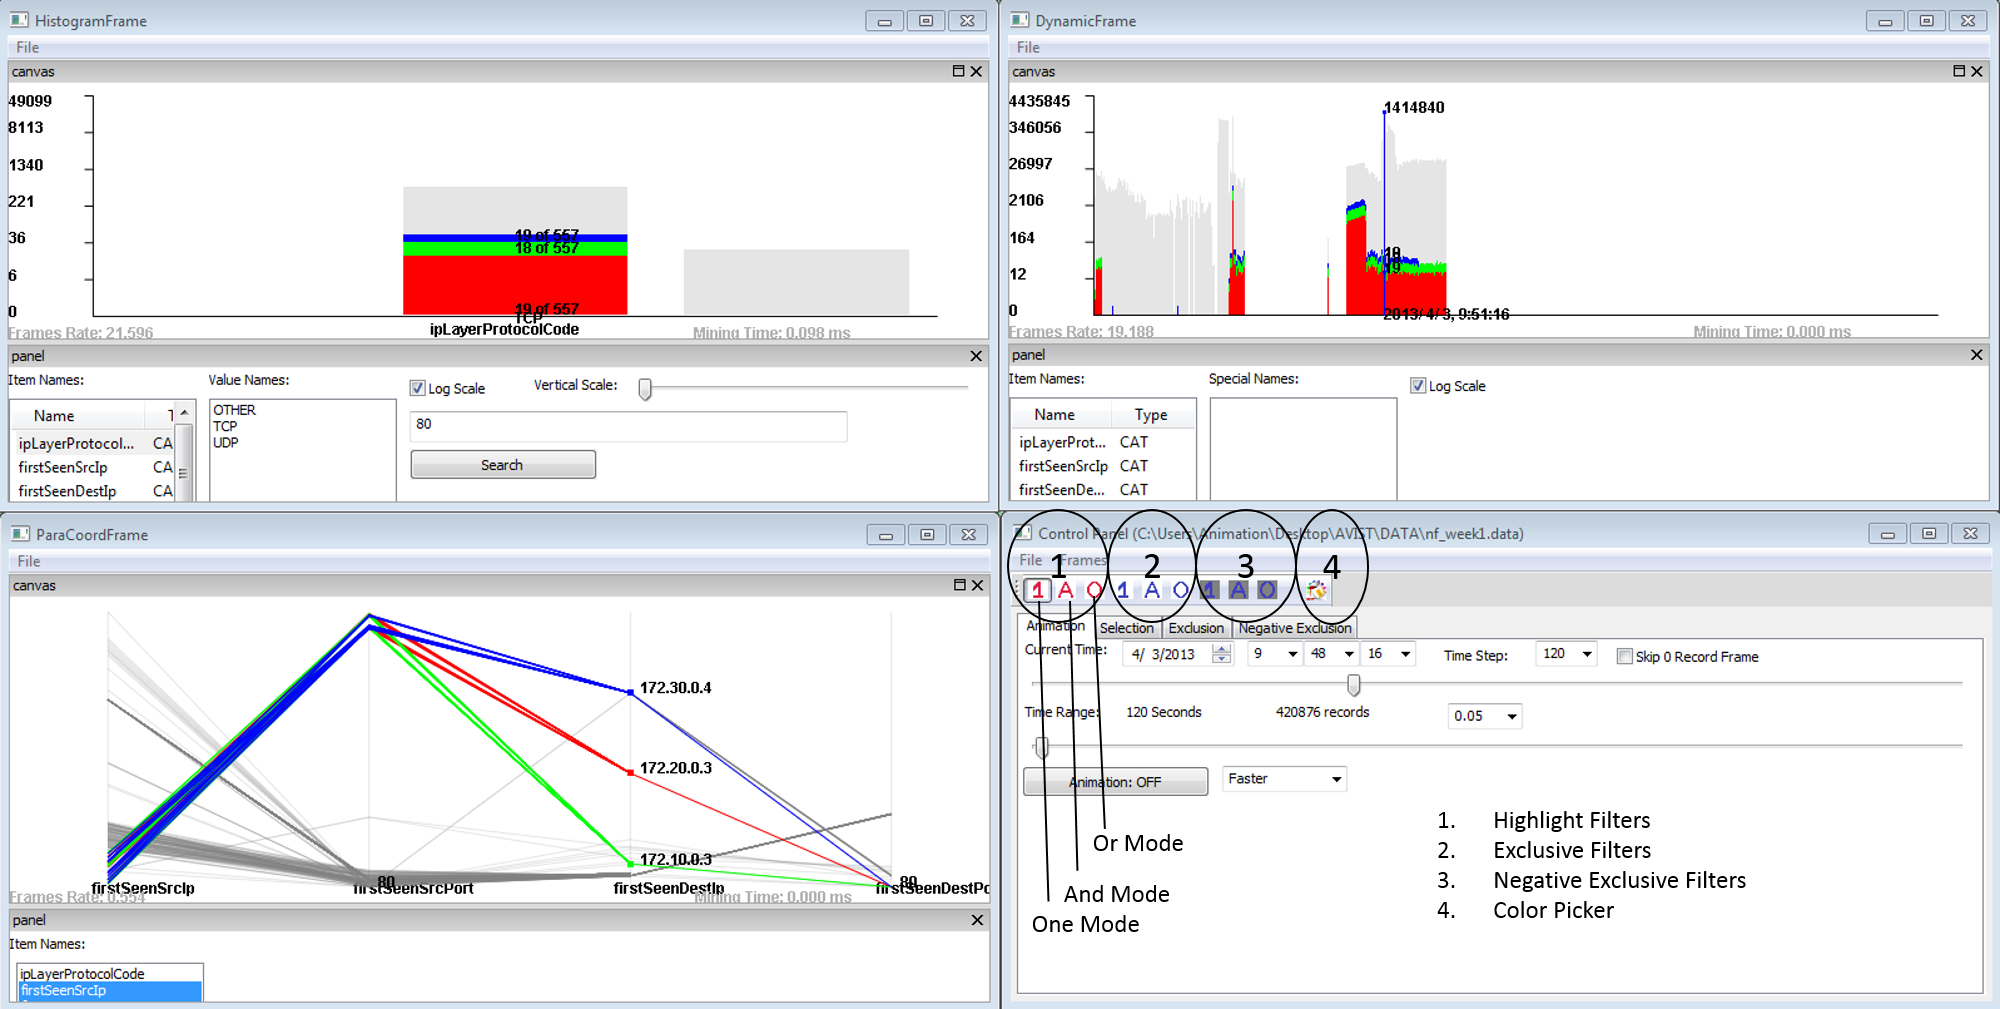
\includegraphics[width=0.8\linewidth]{pic/DataView.png}
%	\parbox[t]{1.0\columnwidth}{\relax
%	}
	%
%	\caption{\label{fig:views}
%		Three data views and control panel of AVIST. The top left is histogram view, top right is dynamic view, bottom left is parallel coordinated view and bottom right is control panel. Each data view is separated into two parts: the canvas for rendering visual primitives and the panel for exploring different data dimensions.}
%\end{figure*}  




\section{Usage Scenario}

In this section, we use two usage scenarios to demonstrate how AVIST support an analyst for visual exploration of big data, to identify hidden patterns, infer and verify new hypothesis.


\subsection{Network Flow Analysis} %Cyber Security Analysis

\begin{figure*}[htb]
	\centering
	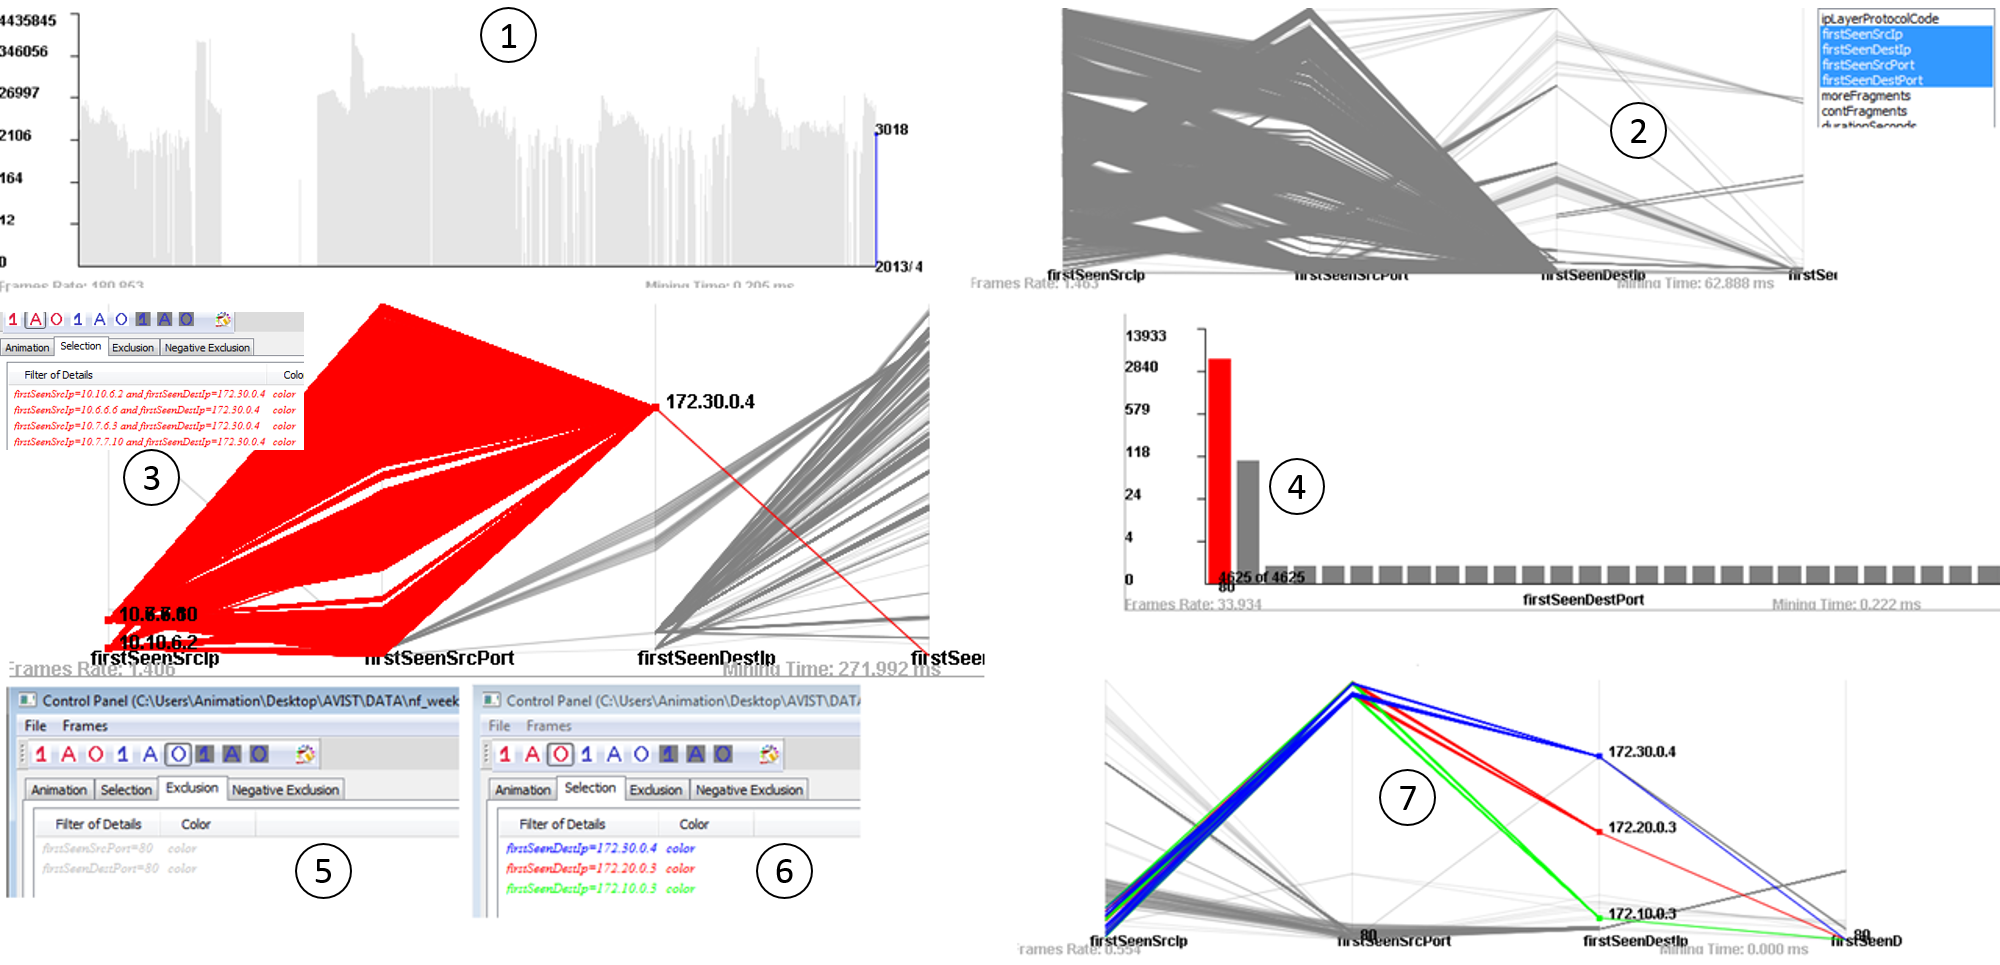
\includegraphics[width=0.9\linewidth]{pic/network2.png}
	\parbox[t]{1.0\columnwidth}{\relax
	}
	%
	\caption{\label{fig:vast}
		This figure shows a usage scenario how AVIST helps analysts for visual exploration of the large network logs. 
		Seven steps are presented in this figure, and Section 6.1 gives more detailed explanations. }
\end{figure*}

\begin{figure*}[htb]
	\centering
	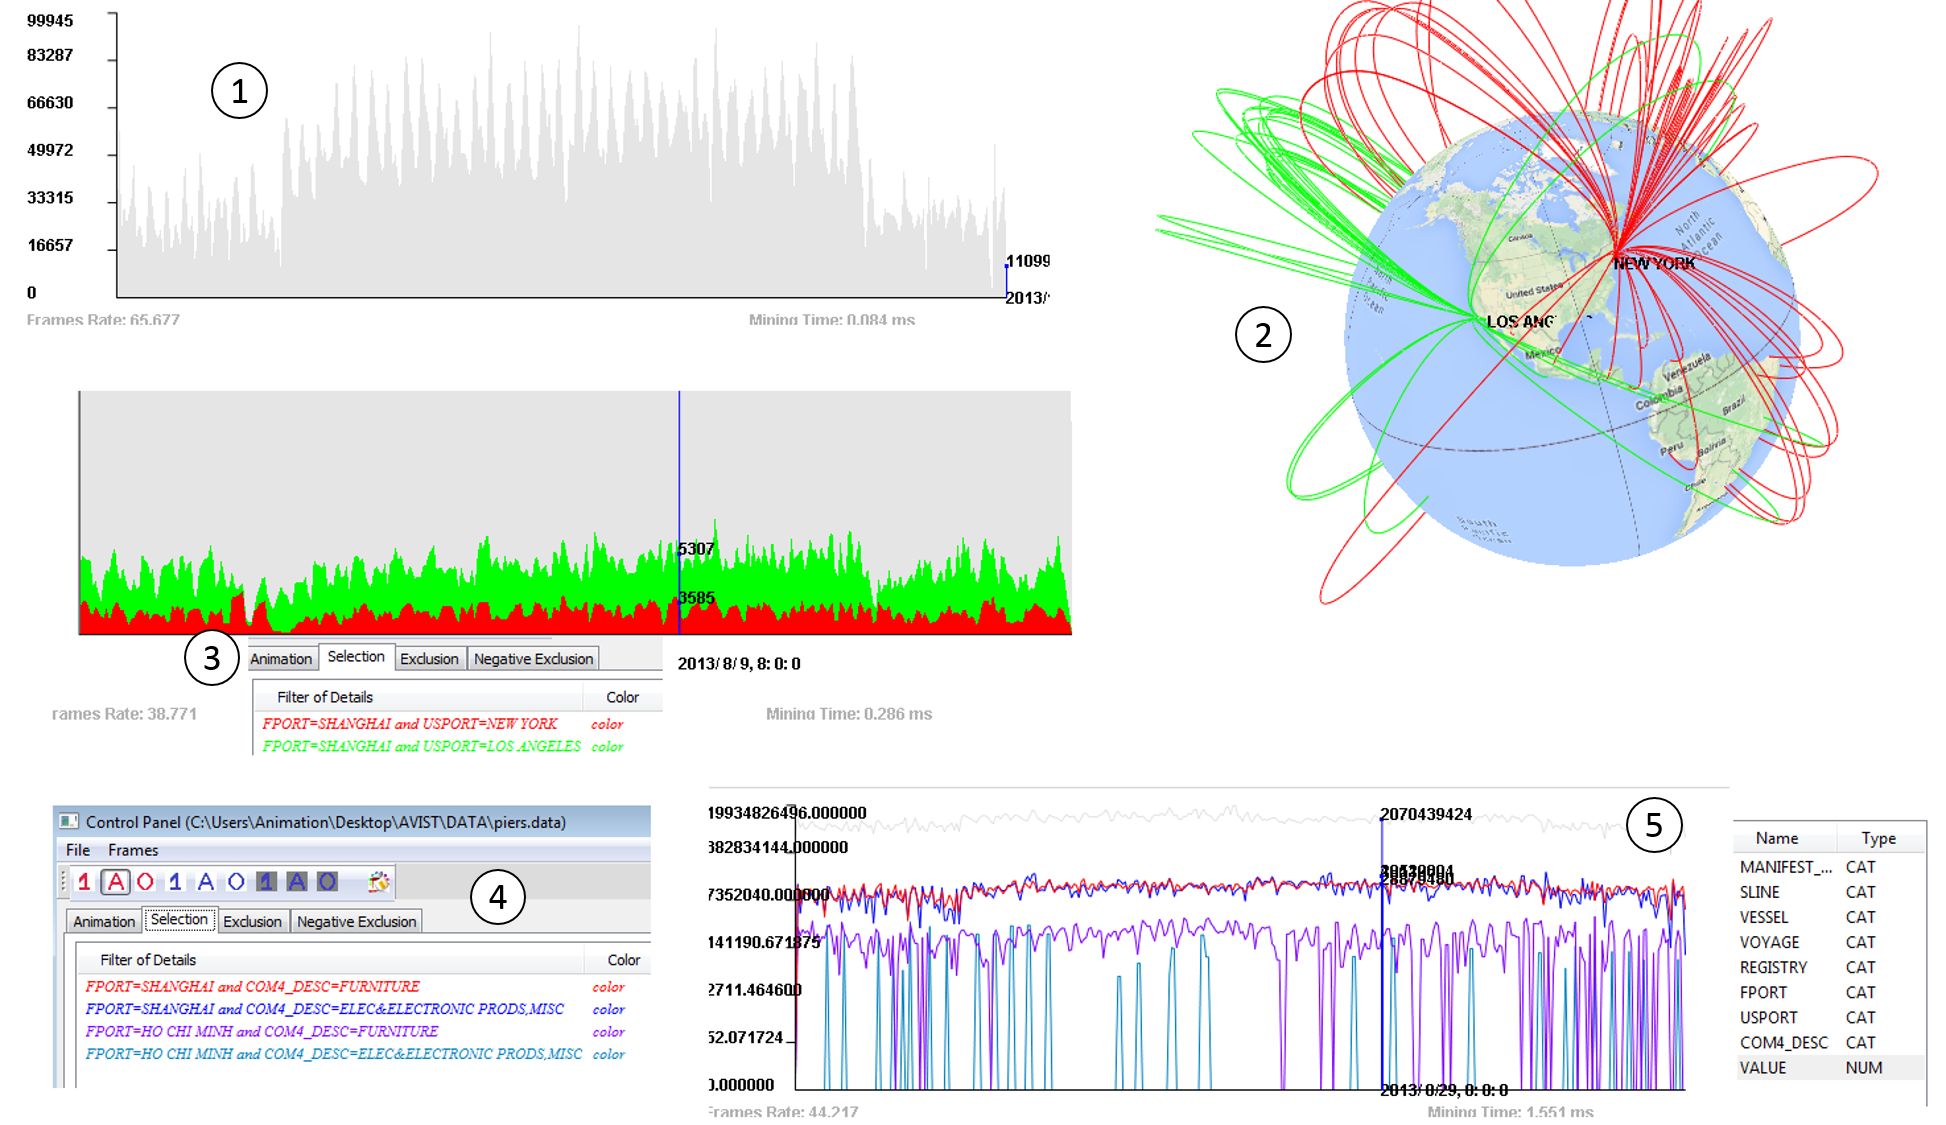
\includegraphics[width=1.0\linewidth]{pic/worldtrade2.png}
	\parbox[t]{1.0\columnwidth}{\relax
	}
	%
	\caption{\label{fig:network}
		This figure shows the usage scenario that analysts use AVIST to visual explore big international trade transactions. The detailed discussions are presented in Section 6.2.}
\end{figure*}

Exploratory visual analysis of network logs is critical for detecting potential cyber threats and network intrusions. VAST 2013 Mini Challenge 3, which targets the analysis of Big Marketing company's network, provides big network traffic logs\footnote{http://vacommunity.org/VAST+Challenge+2013}. One of the datasets is about one week network flow, which includes 46,138,310 records and 16 dimensions.%the total data size is 5.4G

Suppose that Alice is an intelligence analyst. She is assigned to identify the network threats for the Big Marketing company. Firstly, she preprocesses this dataset to obtain the binary data and opens AVIST to load it. Figure~\ref{fig:vast} shows key steps of Alice's visual analytical process. 


\textbf{Data exploration from overview to details.} Firstly, Alice specifies the animation speed and time window size (120 seconds in this example) for automatic animation. The overview of network traffic is visualized in time-series view, shown in subgraph 1. Alice identifies an unusual behavior that the network crashed from 4-2-2013 9:40 am to 4-3-2013 3:26 am. She wants to investigate details before the network crash, so she chooses data dimensions in order of \emph{firstSeenSrcIp}, \emph{firstSeenSrcPort}, \emph{firstSeenDestIp} and \emph{firstSeenDestPort} to generate parallel coordinate plots in subgraph 2. Then she plays animation again and discovers that four source IPs 10.10.6.2, 10.6.6.6, 10.7.6.5, 10.7.7.10 scan the destination IP 172.30.0.4 during 4-2-2013 5:20 am in subgraph 3. 

\textbf{Flexible filtering for revealing hidden patterns.}
Subgraph 4 shows the network traffic distribution of \emph{firstSeenDestPort}. Alice realizes that most of the network records are related with port 80, and she hypothesizes  that these are the normal behavior. She removes these data records with port 80 (subgraph 5) to investigate buried patterns. After the filtering interaction, she plays animation and discovers a port scan activity shown in subgraph 7. She captures this behavior by highlight filters as shown in subgraph 6.  

In this example, Alice iteratively plays animations and tries different filters for identifying potential network threads. She can easily constrains the time and data attributes for capturing any subtle and hidden relationships. Compared with imMens, which preaggregates data before visualization, it cannot provide such flexible interactions, such as cross-domain filtering.
  


\subsection{International Trade Analysis}


Making sense of international trade is important for government and policy makers. With the world economic growth, world trade transactions become large and complex. In this case study, we obtain big international trade transactions from PIERS Global Intelligence Solutions\footnote{https://www.piers.com/}, a private company that provides portfolio analysis for U.S. waterborne trade activity in the world. The dataset is about 2013 US waterborne imports with 10,735,092 records and 10 dimensions. Among 10 dimensions, each data records features the US port code and foreign port code, which illustrates the geospatial information of the dataset.

Suppose that Mike is an economic analyst. He wants to gain insights from the international trade activities. So he  preprocesses and explore this dataset based on AVIST. Figure \ref{fig:network} shows the insights of Mike's visual exploration process.

 
\textbf{Overview exploration.} Mike specifies the time window (86400 seconds or one day) before playing animation. The time-series view shows the overview of the world trades in subgraph 1, which reveals that the activities are clearly separated into four quarters. The second and third quarters has more transactions than others.


\textbf{Hypothesis generation and verification.}
Mike hypothesizes that the international trades may have some spatial patterns. International trades prefer neighboring counties. To verify this, Mike highlights two US ports: Los Angeles (LA) and New York (NY), then he plays animations.
Subgraph 2 shows one snapshot of records with this two ports in virtual globe view, which shows that LA has more trades with pacific countries while NY is more related with Western European. Mike tries to narrow down the data items, which focus on the trades from ShangHai (SH) to LA and NY. He plays animation to refresh the time-series view in subgraph 3. He finds that the trades from SH to LA is roughly twice of trades with NY, which supports  his hypothesis. 

\textbf{Making sense of big data. }
The international trades can character each country's economy. Mike generates four filters to compare the economy of China and Vietnam. He chooses ShangHai port and Ho Chi Minh port for representing these two countries. He emphasizes the trades related about furniture and electronics, as shown in subgraph 4. He is more interested in the money value rather than the number of trades records, so he clicks the value in the listbox and plays animations. Subgraph 5 is the time-series view with four highlighted line charts, which shows that two kinds of trades are more balanced in China, while Vietnam more relies on furniture in its exports. 



\section{Lessons Learned}

 In this section, we summarize some lessons learned for designing and implementing AVIST. We discuss the trade-offs of choosing different technique strategies for big data visual analysis.
 

\begin{itemize}
	\item \textit{Pre-aggregation vs Aggregation on demand}: imMens~\cite{2013-immens} is a pre-aggregation big data visual querying system based on data cube technique. However, it is constraint by 1) long preprocessing time, 2) huge memory requirement (derived data may be larger than original data), and 3) lacking flexible filterings and queries. In contrast, AVIST emphasizes data aggregation on demand, and data storage and computation are done on the GPU to gain performance. Hence, AVIST can provide flexible filtering interactions. We believe that aggregation on demand techniques is a better way for handling the growing datasets.
	
	\item \textit{Row-Oriented vs Column-Oriented}:
	These are two basic data management methods, and both of them have pros and cons. In the ``big data" era, column based method gains more attentions, because columnar databases have two features. Firstly, it has better compression ratio by storing similar things together, and reduce IO cost when transformed from disk to memory. Secondly, it support high level analytical workload very well. While row based database is better for OLTP applications, which supports to  read and write small transactions frequently. The pros of row oriented format includes 1) retrieving small data to find a ``needle in a haystack"; 2) analyzing streaming data with increased datasets. In our paper, we favor row oriented method considering our exploration orientated tasks (e.g., gaining fine-grained data details). 
	
	\item \textit{Exploration-Driven vs Analytical-Driven}:
	 Exploration driven applications emphasize more ``unknow-unknow" knowledge discovery, so they highlight  the data exploration and interaction techniques.
	  However, analytical driven applications focus on ``know-unknow" insight synthesizing, and  they care about integrating statistics and machine learning techniques with human interactions and visual representations.
	  AVIST is an exploration driven tool targeting on visually exploring time series and multi dimensional data. Thus our paper present its design and implementation from data management, computation and exploration aspects.
	   In our case studies, we demonstrate that AVIST can help analysts gain insights,  generate and verify hypotheses.  
	
	\item \textit{Vertical Scaling vs Horizontal Scaling}:
	Performance is a key concern for design big data VA systems. Parallelization is a choice to reduce performance overhead and scale to larger datasets. In this paper, we emphasize the performance gains on a single computer. Thus fully exploiting the GPU resources is our design goal. And our GPU-centric design is constrained by the limited resource of a single node. To handle even bigger datasets, distributed system need be considered. However, distributed systems are designed for long batch jobs. Even they switch the focus to interactive analysis tasks, and redesign distributed frameworks, such as Spark~\cite{Zaharia:2010}. However, these distributed systems are analytical driven, which emphasize on scaling data mining and machine learning from small data into big, rather than exploring the datasets. In our paper, we try to utilize the GPU resources in one computer node to interactively visual exploration of big data, which focus on one computer resource rather than multiple computers.  

	
 
	
\end{itemize}



\section{Conclusions}

 In this paper, we contribute a GPU-centric design for visual exploration of big data. We emphasize the GPU platform for storing and processing data by fully exploiting the GPU resources. In addition, we propose a data dependency graph design to character data computation on the GPU. 
 
 As a proof of concept, we implement AVIST based on our design. We highlight animation and cross-filtering interactions for slicing big data into fine details, and parallel computation for generating visual primitives. The code organization follows MVC pattern, and it shows the detailed GPU data transformation of four data views. 
  
 We demonstrate how AVIST help analysts to gain insights of big data within two usage scenarios.  Lastly, we summarize the lessons learned, discuss the trade-offs of different techniques for designing big data visual analysis systems.  
  



%We admit that this kind of design is limited by GPU memory size, and it can not handle big data scaled to terabyte. The out-of-core technique is our future, which utilizes main memory and focus on data transform between GPU memory and main memory. Better data compression techniques are the potential solutions for scaling big data in GPU.   
 
%$data items = records * dimensions$

%\subsection{Data Dependency Graph}



%// tell the in-situ concept, scientific visualization, dramel

%first identify the design require of the system architecture, then we highlight the GPU based In-Situ Architecture for big data VA system.

%data compression //raw data, meta-data preprocessing

%latency and through  rendering performance GPU In-situ 

%incremental computing Data dependency graph

%\subsection{Requirement Analysis and Design Principle}
%To real time exploratory analysis time-series and high dimensional datasets, 

 














%The main contribution of this paper is the \emph{in-situ}
%We borrow the \emph{in-situ} concept from scientific visualization filed, and present a GPU based in-situ visualization architecture, which features the computing and rendering running simultaneously to reduce I/O costs. To utilize powerful GPU resources,       
 
%In this paper, we presented AVIST system for exploratory visual analysis big data. 
%p1: our contributions
%p2:  cirtical previous design
%p3: continue say our contribution
%p4: limiattions
 



%We presented AVIST system - a GPU based animation visualization toolkit for exploratory visual analysis large time-series and multidimensional dataset.

%p1: contribution what we did, and why it is useful, point 1, point 2, combined together
%p2: future work

%Firstly, analysts can specify animation speed and time window size (120 seconds in this example) to play animation. Dynamic view provides the overview of one week's network flow in subgraph 1. Analysts find there is no any network data during 4-2-2013 9:40 am to 4-3-2013 3:26 am, which  indicates that the whole network had been crushed. To investigate the details, analysts choose source ip and port, destination ip and port to generate parallel coordinate view in subgraph 2. Analysts then play animation again and find unusual pattern in subgraph 3. Analysts identify this pattern's details using highlight filters, and they find that machine 172.30.0.4 was trying to scan three machine during 4-2-2013 5:20 am.  However, visualization of parallel coordinate view are always over-cluttered. In histogram view of subgraph 4, analyst find most of network flow are from port 80. These network flow may be normal to access company's webpage. Analysts apply exclusive filters to remove the network logs, which had access 80 port in subgraph 5. Subgraph 6 shows that analysts use different color to highlight source ips to reveal the port scan behavior in subgraph 7. Figure \ref{fig:views} shows the whole picture of  port scan behavior. After analysts highlight three suspicious ips, they play animation again to identify the behavior distribution in histogram view and dynamic view. They find that the port scan may be a periodical behavior and it happens in TCP transactions. These information may infer analysts next interaction to query more.


\bibliographystyle{abbrv}
%%use following if all content of bibtex file should be shown
%\nocite{*}
\bibliography{template}
\end{document}

